%%%%%%%%%%%%%%%%%%%%%%% file template.tex %%%%%%%%%%%%%%%%%%%%%%%%%
%
% This is a general template file for the LaTeX package SVJour3
% for Springer journals.          Springer Heidelberg 2010/09/16
%
% Copy it to a new file with a new name and use it as the basis
% for your article. Delete % signs as needed.
%
% This template includes a few options for different layouts and
% content for various journals. Please consult a previous issue of
% your journal as needed.
%
%%%%%%%%%%%%%%%%%%%%%%%%%%%%%%%%%%%%%%%%%%%%%%%%%%%%%%%%%%%%%%%%%%%
%
% First comes an example EPS file -- just ignore it and
% proceed on the \documentclass line
% your LaTeX will extract the file if required
\begin{filecontents*}{example.eps}
%!PS-Adobe-3.0 EPSF-3.0
%%BoundingBox: 19 19 221 221
%%CreationDate: Mon Sep 29 1997
%%Creator: programmed by hand (JK)
%%EndComments
gsave
newpath
  20 20 moveto
  20 220 lineto
  220 220 lineto
  220 20 lineto
closepath
2 setlinewidth
gsave
  .4 setgray fill
grestore
stroke
grestore
\end{filecontents*}
%
\RequirePackage{fix-cm}
%
%\documentclass{svjour3}                     % onecolumn (standard format)
%\documentclass[smallcondensed]{svjour3}     % onecolumn (ditto)
%\documentclass[smallextended]{svjour3}       % onecolumn (second format)
\documentclass[twocolumn]{svjour3}          % twocolumn
%
\smartqed  % flush right qed marks, e.g. at end of proof
%
\usepackage{multirow}
\usepackage{color}
\usepackage{graphicx}
\usepackage{amsmath}
\usepackage{enumerate}
\usepackage{subfigure}
\usepackage{booktabs}
\usepackage{float}
\usepackage{graphicx}
\usepackage[colorlinks=true,allcolors=blue]{hyperref}
\usepackage{marvosym}
\usepackage{hyperref}

%
% \usepackage{mathptmx}      % use Times fonts if available on your TeX system
%
% insert here the call for the packages your document requires
%\usepackage{latexsym}
% etc.
%
% please place your own definitions here and don't use \def but
% \newcommand{}{}
%
% Insert the name of "your journal" with
% \journalname{myjournal}
%
\begin{document}

\title{FPGA Acceleration of Secret Sharing for 3D Data Cubes%\thanks{Grants or other notes
%about the article that should go on the front page should be
%placed here. General acknowledgments should be placed at the end of the article.}
}

%\titlerunning{Short form of title}        % if too long for running head

\author{Zi-Ming Wu \and Tao Liu \and Bin Yan\textsuperscript{\Letter} \and Jeng-Shyang Pan \and Hong-Mei Yang
}

%\authorrunning{Short form of author list} % if too long for running head

\institute{Bin Yan\textsuperscript{\Letter} \at
              College of Electronic and Information Engineering, Shandong
              University of Science and Technology, Qingdao, 266590, Shandong,
              People’s Republic of China \\
              \email{yanbinhit@sdust.edu.cn}           %  \\
%             \emph{Present address:} of F. Author  %  if needed
           \and
           Zi-Ming Wu \at
              College of Electronic and Information Engineering, Shandong
              University of Science and Technology, Qingdao, 266590, Shandong,
              People’s Republic of China
}

\date{Received: date / Accepted: date}
% The correct dates will be entered by the editor


\maketitle

\begin{abstract}
Secret sharing can protect the security of important secret information in the network environment. However, the computational complexity and processing delay increase drastically when the secret information contains large amounts of data, such as 3D (three-dimensional) data cubes. In order to improve the efficiency of secret sharing on 3D data cubes, this paper proposes a hardware architecture to accelerate the generation of shares and reconstruction of the secret. The proposed hardware architecture parallelizes the secret sharing process and optimizes on this basis to save large amounts of circuit resources. Simulation results show that this architecture performs secret sharing more than ten times faster than the software implementation. This study enables the secret sharing of 3D data cubes, which protect large amounts of data information throughout the process and allows complete reconstruction of 3D data cubes. To be able to handle secrets without decoding them, we then extend the hardware architecture to the four basic processes of multi-party computation, demonstrating the feasibility of the structure and providing preliminary research tools for the effective implementation of multi-party computation.
\keywords{Parallel processing \and 3D data cubes \and Secret sharing \and FPGA \and Multi-party computation}
\end{abstract}

\section{Introduction}\label{Sec_intro}

As a carrier of information, 3D data cubes can store more information than 2D (two-dimensional) images and are widely used in various fields, such as medical 3D images, seismic 3D exploration and VR (virtual reality). At the same time, in order to ensure the confidentiality and effectiveness of information in the transmission process, people use cryptography to encrypt the data\cite{2011Contemporary}. But when it comes to situations where the data needs to be handed over to others for processing, there is a risk of revealing secrets. For example, If people's medical records are not encrypted at the time of their visit, some private medical records could be exposed and victims with certain diseases could lose their jobs. People cannot encrypt their information if they want to seek medical treatment. To solve such problems, secret sharing and multi-party computation have been proposed and have been an important area of research for many years\cite{chanu2019survey}.

Shamir and Blakley introduced a $(t, n)$-threshold secret sharing scheme in 1979\cite{shamir1979share,mceliece1981sharing,blakley1979safeguarding}. This scheme divides the secret into $n$ shares and distributes them to $n$ users. Each user gets at least one share. Each share alone will not reveal any secret information. Also, these shares are delivered to the users through a private channel, so the users are not aware of other people's information among themselves. When $t$ shares are assembled, the secret reconstruction can be performed by Lagrangian interpolation. This encryption has become an important method for designing secure protocols such as threshold signatures\cite{wang2014simulatable}, key management\cite{hanaoka2002hierarchical,liu2017security}, multi-party computation\cite{halpern2004rational,pilaram2021efficient,blanton2020improved}, electronic voting schemes\cite{iftene2007general}, QR codes\cite{PAN2022103405,PAN2021104049,article} and access control\cite{han2012attribute}. Since a large amount of computation is required for secret sharing, a limit on the amount of data is needed to ensure the efficiency of encryption. 2D images contain less information than 3D data cubes, so this encryption method is widely used for 2D information encryption.

Thien and Lin used secret sharing scheme to share 2D secret images for the first time\cite{thien2002secret}. However, the calculation process is slower and wastes computing memory compared to Boolean sharing. Then, on this basis a series of secret sharing schemes are proposed to deal with different situations, which can be summarized as follows: Boolean operation sharing\cite{kabirirad2019improvement,kumar2022extending}, progressive sharing\cite{xiong2021cp,prasetyo2019xor}and scalable sharing\cite{wang2006secret}. These schemes are proposed to solve the problem of information security in different situations, but only for information with a small amount of data. Since the byte size of each image pixel is fixed, one puts the secret sharing on a finite field for polynomial computation\cite{beimel1994universally,hansen2017secret}. F. Xing achieved lossy recovery of 2D images by putting the sharing of 2D secret images on a finite field for polynomial operations, and the computational complexity is $O\left(n^{3}\right)$\cite{xing2022information}. C. Qin realized the secret sharing process of 2D images on $2^{8}$ field and realized the complete recovery of 2D images\cite{qin2021reversible}. However, the computational complexity of the multiplication operation on the $2^{8}$ field is higher than that on the 251 field as $O\left(n^{4}\right)$. 3D data cubes have increased in dimensionality compared to 2D data cubes and require more computation. {\color{red}Compared to CPU, FPGA(Field Programmable Gate Array) can increase computing efficiency by parallel processing. This means that it can process multiple data at the same time and perform different tasks simultaneously. Thus, the processing speed of the whole system is accelerated.} So FPGA is considered to increase the speed of sharing.

Stangl J. used FPGA to share files with the different number of storage bytes\cite{stangl2018fast}. The relationship between secret file bit width and sharing efficiency is investigated to provide the possibility of implementing secret sharing of 3D data cubes. Patel uses FPGA to accelerate the MPC process in the public cloud. The bit depth of the subject information in this process is 1\cite{patel2020arithmetic}. This restricts its usage in sharing images with higher bit depth, such as gray-scale images.

From the above study, secret sharing can encrypt the data without revealing any information and can recover the data losslessly. However, most of the current secret sharing is implemented in software and reduces the computational effort by setting a lower threshold. This results in a low number of generated shares. To address these issues, we use parallel processing of FPGA to accelerate the secret sharing process to generate more shares in less time.


The contribution of this work can be highlighted as follow:
\begin{enumerate}
	\item Using FPGA to accelerate polynomial multiplication, enabling secret sharing of 3D data cubes.
	\item Extending this process to the four basic processes of multi-party computation provides a preliminary research tool for the effective implementation of multi-party computation.
\end{enumerate}

This paper is organized as follows. In section~\ref{Sec_relatedworks}, we describe the background knowledge related to our proposal. Section~\ref{Sec_proposed} gives the general scheme. Section~\ref{Sec_Multi-party} extends the process to the four basic processes of multi-party computation. Section~\ref{Sec_experiments} presents experimental results and discussions. Finally, we conclude this paper in section~\ref{Sec_conclusion}.

\section{Related background}\label{Sec_relatedworks}

In this section, we review existing research and techniques to provide a knowledge base for our work. The basic concepts of 3D data cubes, secret sharing, finite field, and multi-party computation are introduced.

\subsection{3D data cubes }\label{(2,2)-VC}

3D data cubes can be considered as a stacking of 2D images, and are more substantial in terms of data volume than 2D images.

The main object of this paper is the 3D data cubes. Three slices of a 3D data cubes are shown in Fig. \ref{fig01}. It is assumed that the original 3D data cubes consist of $K$ layers of 8-bit grayscale images of size $M\times W$.

\begin{figure}[!htb]
	\begin{center}
		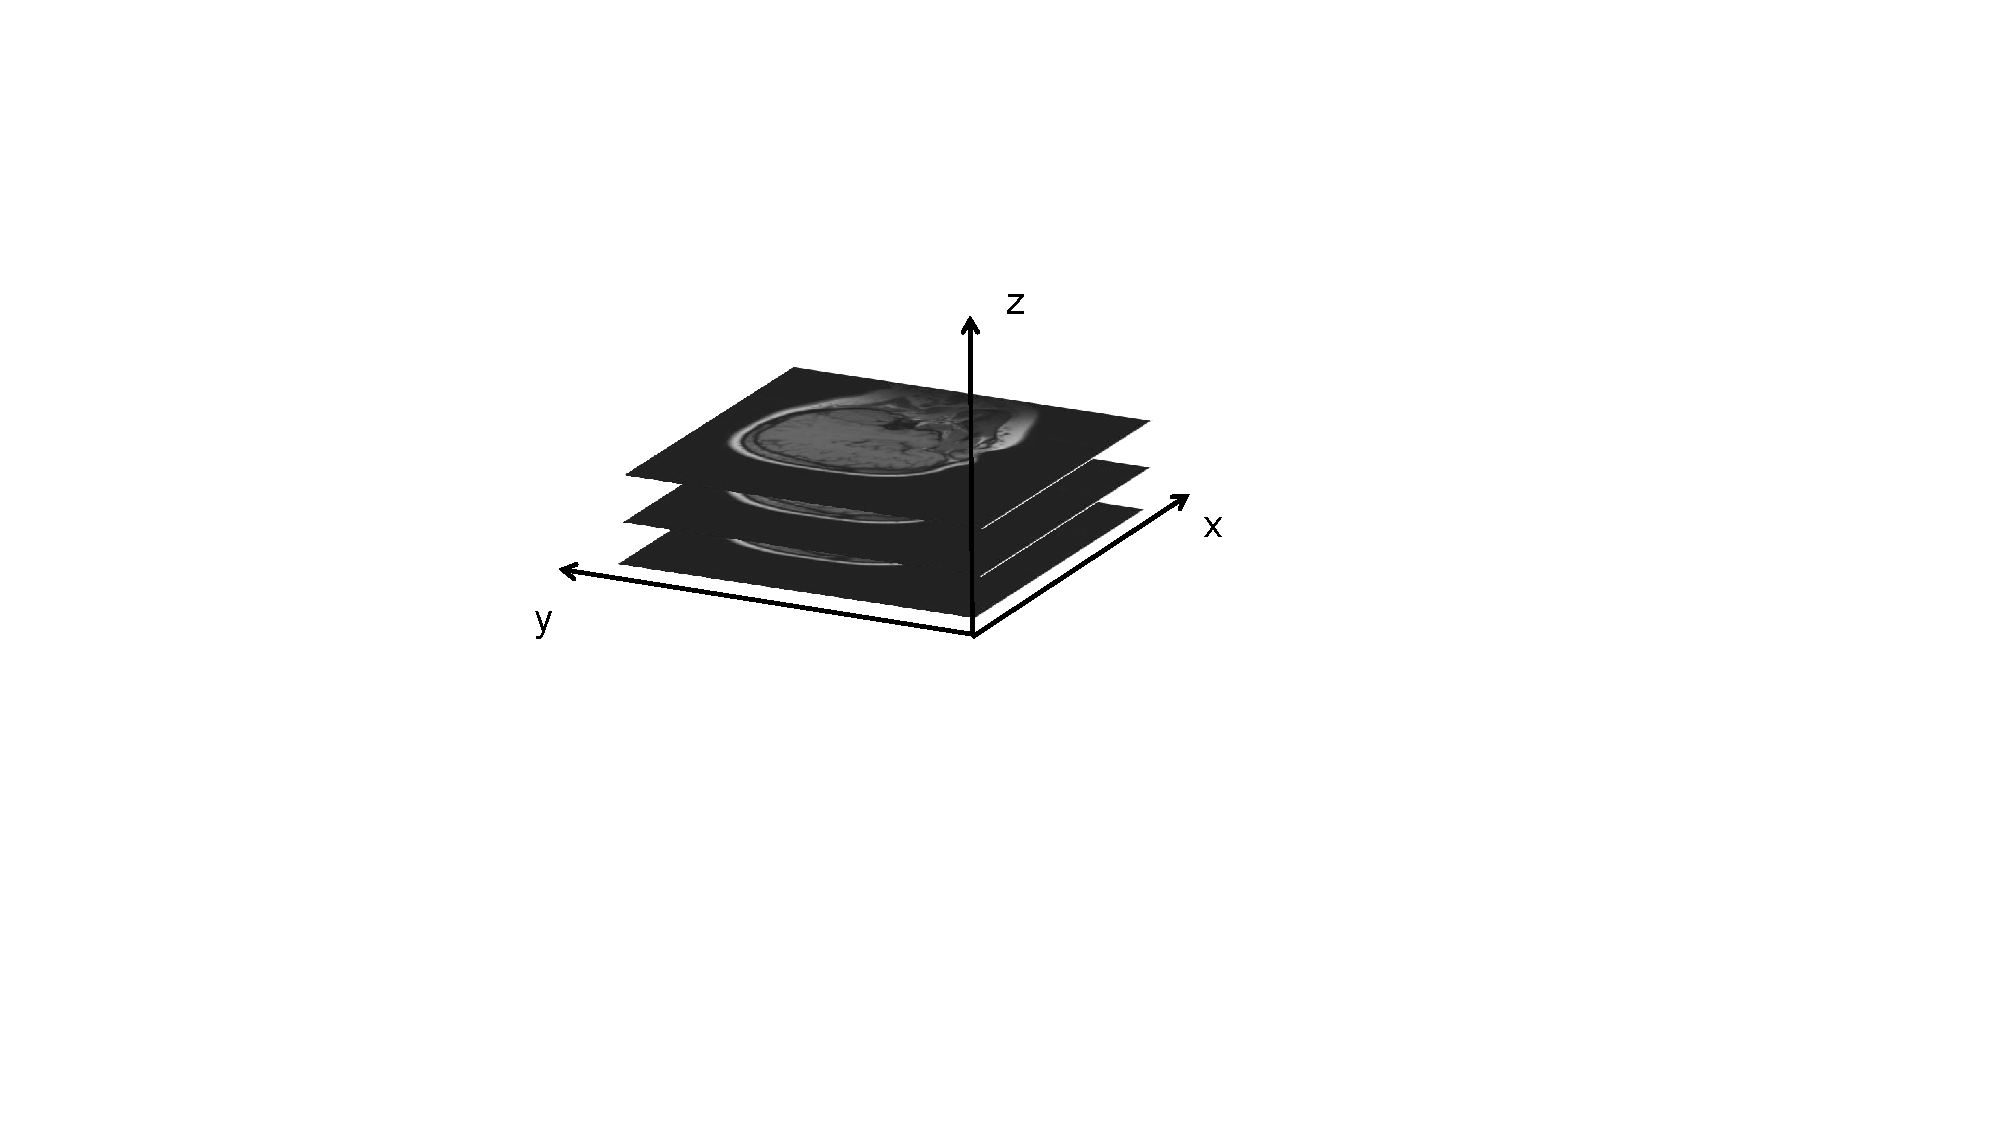
\includegraphics[width=4cm]{imageslice.eps}\\
		\caption{3D data cubes slices}
		\label{fig01}
		\vspace{-5.0em}
	\end{center}
\end{figure}

\subsection{Shamir secret sharing }\label{(2,2)-VC}

Shamir proposed a $(t, n)$-threshold scheme by splitting a secret into multiple shares for protection:

\begin{enumerate}
	\renewcommand{\labelenumi}{(\theenumi)}
	\item By splitting a secret into several copies allows multiple people to work together to manage the recovery of the secret.
	\item When more than $t$ shares can be recovered as the secret, but less than $t$ shares cannot be recovered as the secret.
\end{enumerate}

Secret sharing is divided into a share generation phase and a secret reconstruction phase. All computations are performed in the finite field $GF(p)$, where $p$ is a prime number which is greater than the maximum value in $n$ and secret.

In the share generation phase, we choose $n$ different elements $x_{1}, x_{2},\dots,$ and $x_{n}\left(x_{i} \geq 0\right)$ in $GF(p)$ to calculate $f\left(x_{1}\right), f\left(x_{2}\right), \cdots,$ and $f\left(x_{n}\right)$
\begin{equation}\label{eq1}
f(x_{i} )=\left(a_{0}+a_{1} x_{i}+\cdots+a_{t-1} x_{i}^{t-1}\right) \bmod p,
\end{equation}where $a_{0}$ is the secret and $a_{1},a_{2},\cdots,a_{t-1}$ are the random numbers uniformly sampled from $GF(p)$. Thus we get $n$ shares, each share and the corresponding $x_{i}$ is managed by a single user.

In the secret reconstruction phase, one collects any $t$ or more shares and the corresponding $x_{i}$. The secret can be reconstructed by Lagrangian interpolation
\begin{equation}\label{eq1}
F(x)=\sum_{i=1}^{n}\left(f\left(x_{i}\right) \prod_{\substack{1 \leq \omega \leq n \\ \omega \neq i}} \frac{x-x_{\omega}}{x_{i}-x_{\omega}}\right) \bmod p.
\end{equation}When $x$ takes the value of 0, the secret $a_{0}$ can be expressed as
\begin{equation}\label{eq1}
a_{0}=\sum_{i=1}^{n}\left(f\left(x_{i}\right) \prod_{\substack{1 \leq \omega \leq n \\ \omega \neq i}} \frac{-x_{\omega}}{x_{i}-x_{\omega}}\right) \bmod p.
\end{equation}
\subsection{GF finite field}\label{(2,2)-VC}

In cryptography, the finite field $GF(p)$ is a very important field, where $p$ is a prime number. Only if $p$ is taken to be prime can all elements of the set be guaranteed to have additive and multiplicative inverse elements.

Since 256 is not a prime number, we can only obtain the largest prime number less than 256 as 251. So people often directly determine the number greater than or equal to 251 as 250. This is often done in image processing, but then the image is not fully recovered\cite{article13}.

To avoid the loss of pixel data from 251 to 256 introduce $GF(p^{n})$. Let $p$ be 2 and $n$ be 8, that is $GF (2^{8})$.
The calculation characteristics of this field are as follows.


\subsubsection{Polynomial addition and subtraction}\label{subsec_NC-BPDVC_framework}

Suppose there are two polynomials $f(x)$ and $g(x)$

\begin{equation}\label{eq1}
f(x)=x^{5}+x^{4}+x^{3}+x\quad and\quad g(x)=x^{5}+x^{2}.
\end{equation}
The addition of these two polynomials over $GF (2^{8})$ can be expressed as

\begin{equation}\label{eq1}
\begin{aligned}
f(x)+g(x) & =\left(x^{5}+x^{4}+x^{3}+x\right)+\left(x^{5}+x^{2}\right) \\
& =x^{4}+x^{3}+x^{2}+x.
\end{aligned}
\end{equation}Converting the polynomial in the equation to binary format gives
\begin{equation}\label{eq1}
f(x)+g(x)=00111010 \oplus 00100100=00011110.
\end{equation}

It follows that the addition and subtraction of polynomials are equivalent to the binary XOR (exclusive OR) operation.

\subsubsection{Polynomial multiplication}\label{subsec_NC-BPDVC_framework}

The principle of multiplication is that all numbers in binary can be obtained by dissimilarity with  0x01, 0x02, 0x04, 0x08, 0x10, 0x20, 0x40, 0x80\cite{article12}. For example, $x\times 10101101$ can be expressed as
\begin{equation}
x \times(0\mathrm{x} 80 \oplus0\mathrm{x} 20\oplus0\mathrm{x} 08\oplus0\mathrm{x} 04\oplus0\mathrm{x} 01).
\end{equation}
So we only need to calculate the value of $x\times0\mathrm{x}01,x\times 0\mathrm{x}02,\dots,x\times0\mathrm{x}80$, then all the multiplication results can be obtained.

To calculate multiplication in a finite field, we must first determine an 8-degree irreducible polynomial on $GF (2^{8})$. After referring to the AES algorithm, we determine it as
\begin{equation}
x^{8}+ x^{4}+ x^{3}+ x + 1.
\end{equation}
When the highest bit of the value is 1, the maximum value of the field will be exceeded if the value is shifted further left. So after the shift operation, the value needs to XOR $0\mathrm{x}1 b$.

The multiplication of these two polynomials on $GF (2^{8})$ can be expressed as
\begin{equation}\label{eq1}
f(x) \times g(x)=\left(x^{5}+x^{4}+x^{3}+x\right) \times\left(x^{5}+x^{2}\right).
\end{equation}Separate $g(x)$ by bit gives
\begin{equation}\label{eq1}
f(x) \times g(x)=0 \mathrm{x}  3 a \times 0 \mathrm{x}  24=0 \mathrm{x}  3 a \times(0 \mathrm{x}  04 \oplus 0 \mathrm{x}  20).
\end{equation}Converts a multiplication operation to a shift operation
\begin{equation}\label{eq1}
\begin{aligned}
0 \mathrm{x} 3 a \times 0 \mathrm{x} 04 & =00111011<<2=11101000, \\
0 \mathrm{x} 3 a \times 0 \mathrm{x} 20 & =(00111011<<5) \oplus 0 \mathrm{x} 1 b \\
& =00000001.
\end{aligned}
\end{equation}The final result of multiplying two polynomials together can be expressed as
{\color{red}
\begin{equation}\label{eq1}
\begin{aligned}
f(x) \times g(x) & =(0 \mathrm{x} 3 a \times 0 \mathrm{x} 04)\oplus (0 \mathrm{x} 3 a \times 0 \mathrm{x} 20) \\
& =11101001.
\end{aligned}
\end{equation}
}
\subsection{Multi-party computation}\label{(2,2)-VC}

Multi-party computation allows algorithmic computations to be performed directly on the share, and secret reconstruction is performed to obtain the secret for which the same computation has been performed.

This feature is important for protecting the security of information, mainly by taking advantage of the fact {\color{red}that secret sharing is linear encryption.} In this process it is possible to protect secret information from being leaked.

\subsubsection{Addition process and multiplication process}\label{subsec_NC-BPDVC_framework}

In the addition process and multiplication process, a constant operation can be added to the shares. The process can be expressed as
\begin{equation}
\begin{array}{l}
f\left(x_{i}\right) \oplus n=\left(a_{0} \oplus n\right) \oplus a_{1} x_{i} \oplus \ldots \oplus a_{t-1} x_{i}^{t-1},\\
f\left(x_{i}\right) n=\left(a_{0} n\right) \oplus\left(a_{1} n\right) x_{i} \oplus \ldots \oplus \left(a_{t-1} n\right) x_{i}^{t-1}.
\end{array}
\end{equation}In these process, $n$ represents the constant, ${a}_{0}$ represents the secret, and $f\left(x_{i}\right)$ represent shares. The reconstruction of the secret can be done by Lagrangian interpolation. The obtained secret will perform the same constant operation.

\subsubsection{Double shares addition process}	

In the double shares addition process, the two shares can be added together and the result of the corresponding secret addition is obtained after decryption. The two shares generation can be expressed as
\begin{equation}
\begin{array}{l}
f_{1}\left(x_{i}\right)=s_{j} \oplus a_{1} x_{i} \oplus a_{2} x_{i}^{2} \oplus \ldots a_{t-1} x_{i}^{t-1}, \\
f_{2}\left(x_{i}\right)=d_{j} \oplus b_{1} x_{i} \oplus b_{2} x_{i}^{2} \oplus \ldots b_{t-1} x_{i}^{t-1}.
\end{array}
\end{equation}In this equation ${s}_{j}$ represents the first secret, ${d}_{j}$ represents the second secret, $f_{1}\left(x_{i}\right)$ represents the first share, $f_{2}\left(x_{i}\right)$ represents the second share, and the two shares are superimposed additively to obtain

\begin{equation}
f_{1}\left(x_{i}\right) \oplus f_{2}\left(x_{i}\right)=\left(s_{j} \oplus d_{j}\right) \oplus \ldots \oplus\left(a_{t-1} \oplus b_{t-1}\right) x_{i}^{t-1}.
\end{equation}

The polynomial generated after the additive superposition remains a polynomial whose number does not exceed $t-1$ times, so it can be directly reconstructed by using Lagrange interpolation. The recovery process is shown in Fig. \ref{fig02}.

\begin{figure}[!htb]
	\begin{center}
		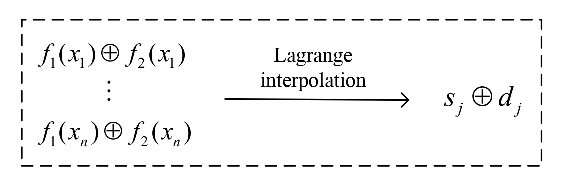
\includegraphics[width=8.5cm]{DAP.eps}\\
		\caption{Double shares addition process}
		\label{fig02}
		\vspace{-2.0em}
	\end{center}
\end{figure}
\subsubsection{Double shares multiplication process}		

The double shares multiplication process can be expressed as
\begin{equation}
f_{1}\left(x_{i}\right) f_{2}\left(x_{i}\right)=\left(s_{j} d_{j}\right) \oplus \ldots \oplus\left(a_{t-1} b_{t-1}\right) x_{i}^{2 t-2}.
\end{equation}

After the multiplicative superposition of the two shares, the polynomial generated is at most $2t-2$ times, and the number of times is completely random. So it cannot be recovered directly by Lagrange interpolation. Therefore, it is necessary to generate polynomials with at most $t-1$ times after the second sharing, and then recover them by Lagrange interpolation. The recovery process is shown in Fig. \ref{fig03}.

\begin{figure}[!htb]
	\begin{center}
		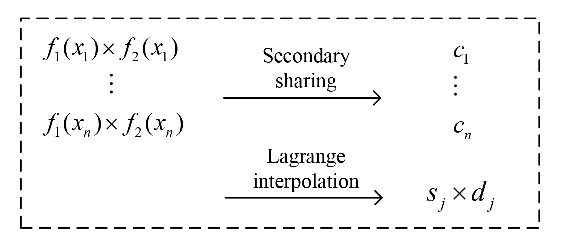
\includegraphics[width=8cm]{DMP.eps}\\
		\caption{Double shares multiplication process}
		\label{fig03}
		\vspace{-2.0em}
	\end{center}
\end{figure}

Respectively, using the multiplicatively superimposed values $f_{1}\left(x_{i}\right)\times  f_{2}\left(x_{i}\right)$ as secrets to regenerate the subshares $
\mathrm{\mathit{c} }_{1 \mathrm{i}}, \mathrm{\mathit{c} }_{2 \mathrm{i}}, \ldots, \mathrm{\mathit{c} }_{n \mathrm{i}}$. The subshares are then linearly superimposed by the recombination coefficients to obtain the secondary shares after sharing $\mathrm{\mathit{c} }_{1}, \mathrm{\mathit{c} }_{2}, \ldots, \mathrm{\mathit{c} }_{n}$. This process can be expressed as
\begin{equation}
\left\{\begin{array}{c}
c_{1}=\alpha_{1} c_{11}+\alpha_{2} c_{21}+\cdots+\alpha_{n} c_{n 1} \\
c_{2}=\alpha_{1} c_{12}+\alpha_{2} c_{22}+\cdots+\alpha_{n} c_{n 2} \\
\vdots \\
c_{n}=\alpha_{1} c_{1 n}+\alpha_{2} c_{2 n}+\cdots+\alpha_{n} c_{n n}.
\end{array}\right.
\end{equation}
\section{Proposed scheme}\label{Sec_proposed}

Our scheme can be divided into a share generation phase and a secret reconstruction phase. The algorithm is divided into different modules to build parallel circuits, achieving secret sharing of 3D data cubes on the $GF (2^{8})$ field.

\subsection{Share generation phase}\label{subsec_NC-BPDVC_framework}

In the share generation phase, the data of the 3D data cubes are first imported into the data processing module for data pre-processing. In this module, all data are arranged as one-dimensional data. After processing the data, they are sequentially imported into the SGM (share generation module) for polynomial computation. Then final shares are generated. This is shown in Fig. \ref{fig04}.

\begin{figure*}
	\begin{center}
	% Use the relevant command to insert your figure file.
	% For example, with the graphicx package use
	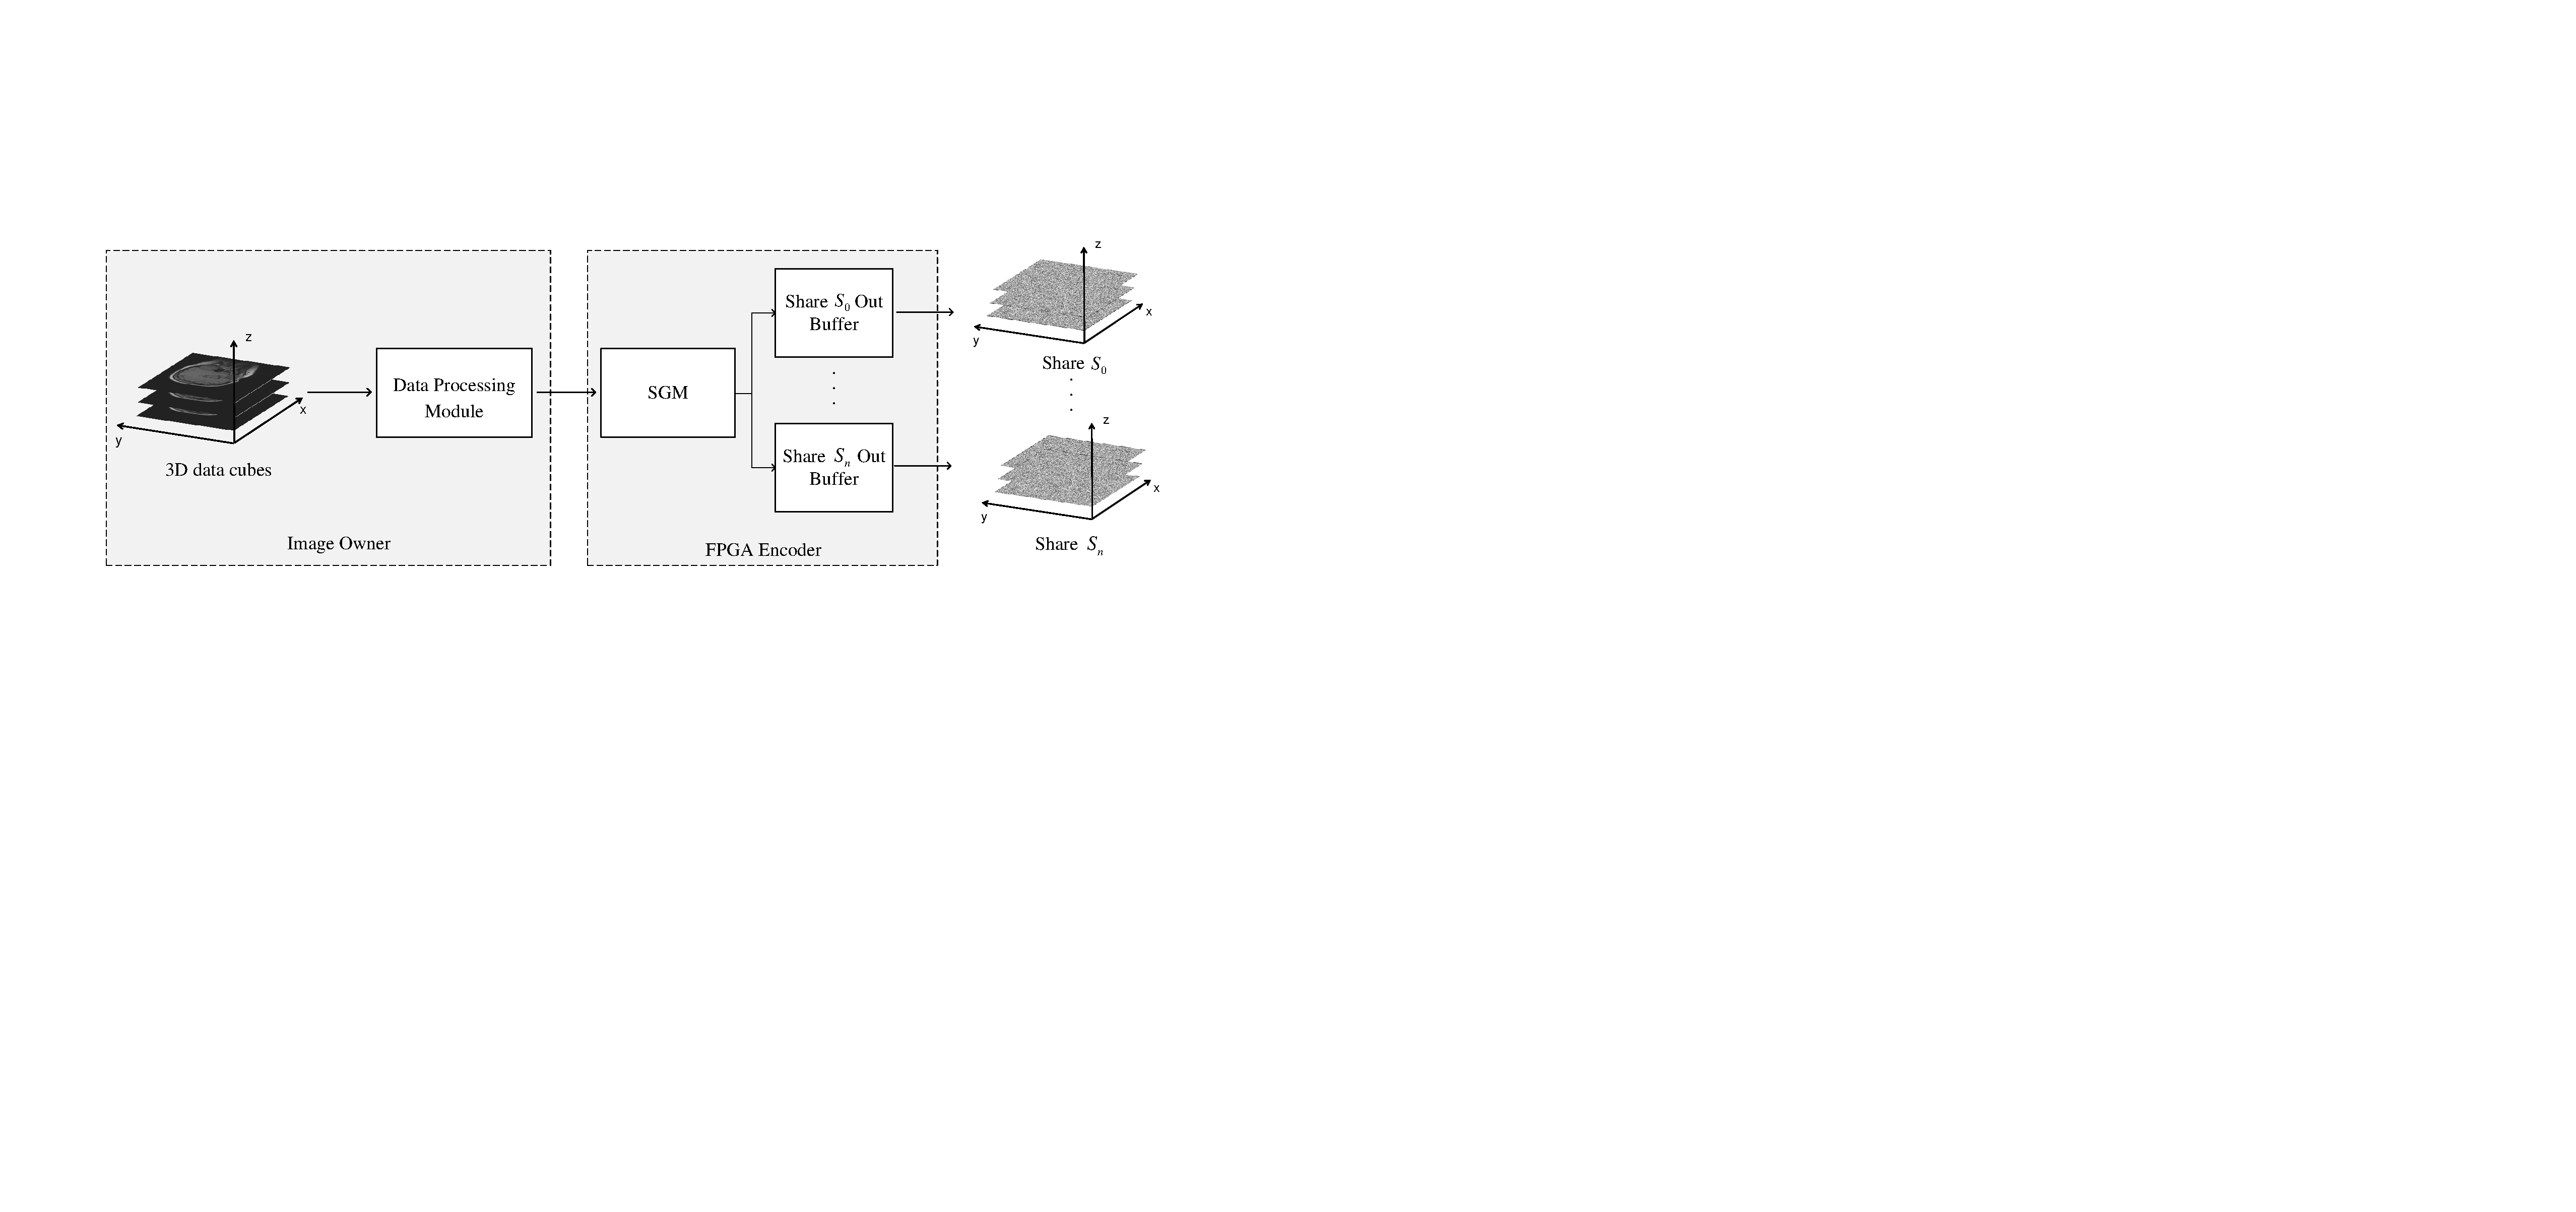
\includegraphics[width=0.85\textwidth]{SGM_liu.eps}
	% figure caption is below the figure
	\caption{{\color{red}Share generation phase}}
	\label{fig04}       % Give a unique label\
	\vspace{-2.0em}
	\end{center}
\end{figure*}

\subsubsection{Share generation module}\label{subsec_NC-BPDVC_framework}

This module performs secret sharing for each data sample in the 3D data cubes sequentially. The secret data are represented by $a_{0}$ and a polynomial of order $t-1$ is constructed for each data.The coefficients $a_{1},a_{2},\cdots,a_{t-1}$ are randomly generated. Thus, each data can generate $n$ shares by setting $x_{i}$ in advance, where $p(x)$ is set as an irreducible polynomial. The $i$-th share is

\begin{equation}
f(x_{i}) =\left(a_{0}  \oplus a_{1} x_{i} \oplus \cdots \oplus a_{t-1} x_{i}^{t-1}\right) \bmod p(x).
\end{equation}The degree of polynomials and the threshold $t$ are positively correlated. To understand the specific characteristics of Shamir secret sharing, the (3,3)-threshold shares generation formula is established as
\begin{equation}
f\left(x_{i}\right)=\left(a_{0}\oplus a_{1} x_{i}\oplus a_{2} x_{i}^{2}\right) \bmod p(x).
\end{equation}After randomly generating three groups of $a_1$ and $a_2$, the share generation equation of 162 as a secret can be expressed as
\begin{equation}
\left\{\begin{array}{l}
f\left(x_{1}\right)=\left(162\oplus 2 x_{1}\oplus 4 x_{1}^{2}\right) \bmod p(x) \\
f\left(x_{2}\right)=\left(162\oplus 2 x_{2}\oplus 4 x_{2}^{2}\right) \bmod p(x) \\
f\left(x_{3}\right)=\left(162\oplus 2 x_{3}\oplus 4 x_{3}^{2}\right) \bmod p(x)
\end{array}\right..
\end{equation}Take $x_{i} $ as 2, 4 and 6 respectively and substitute them into the calculation, the calculation process can be expressed as

\begin{equation}
\left\{\begin{array}{l}
162 \oplus 2 \times 2 \oplus 4 \times 2^{2}=182 \\
162 \oplus 2 \times 4 \oplus 4 \times 4^{2}=234 \\
162 \oplus 2 \times 6 \oplus 4 \times 6^{2}=254
\end{array}\right..
\end{equation}

A complete computation process shows that the process of generating the shares is processed in the same way for each secret data. So the parallelism of FPGA can be considered to pipeline this process.

The SGM is mainly a circuit consisting of random number input ROM, $x_{i}$ input ROM, PMM (polynomial multiplication module), and XOR module.

The random numbers and $x_{i}$ are stored in advance in ROM. The values can be passed in directly by calling the driver address, which reduces the circuit running time. The efficiency of the calculation is improved by parallelizing the different multiplication processes. {\color{red}When generating a share, $x_{i}$ is simultaneously passed into different PMM with $a_{1}$ and $a_{2}$ for computation respectively. However, $a_{1}x_{i}$ and $a_{2}x_{i}^{2}$ have different computations, and $a_{2}x_{i}^{2}$ requires a larger computation step. In order to ensure that the computed results reach the XOR module for computation at the same time, the delay module needs to be added.} The Fig. \ref{fig05} shows the circuit diagram when generating a share.

\begin{figure}[!htb]
	\begin{center}
		\includegraphics[width=8.5cm]{SGU.eps}\\
		\caption{Structure of the SGM}
		\label{fig05}
		\vspace{-2.0em}
	\end{center}
\end{figure}

When the processing object is a 3D data cubes, it is difficult to store the corresponding amount of data in ROM because of the huge data of the 3D data cubes. As the threshold continues to increase, there are more and more PMM in the circuit. This wastes a lot of circuit resources.

So it is necessary to find a way to reduce the circuit resources of the PMM. In order to reduce the resources occupation and increase the speed of synthesis, cyclic multiplication is considered to design the circuit. As shown in Fig. \ref{fig06}.

\begin{figure}[!htb]
	\begin{center}
 		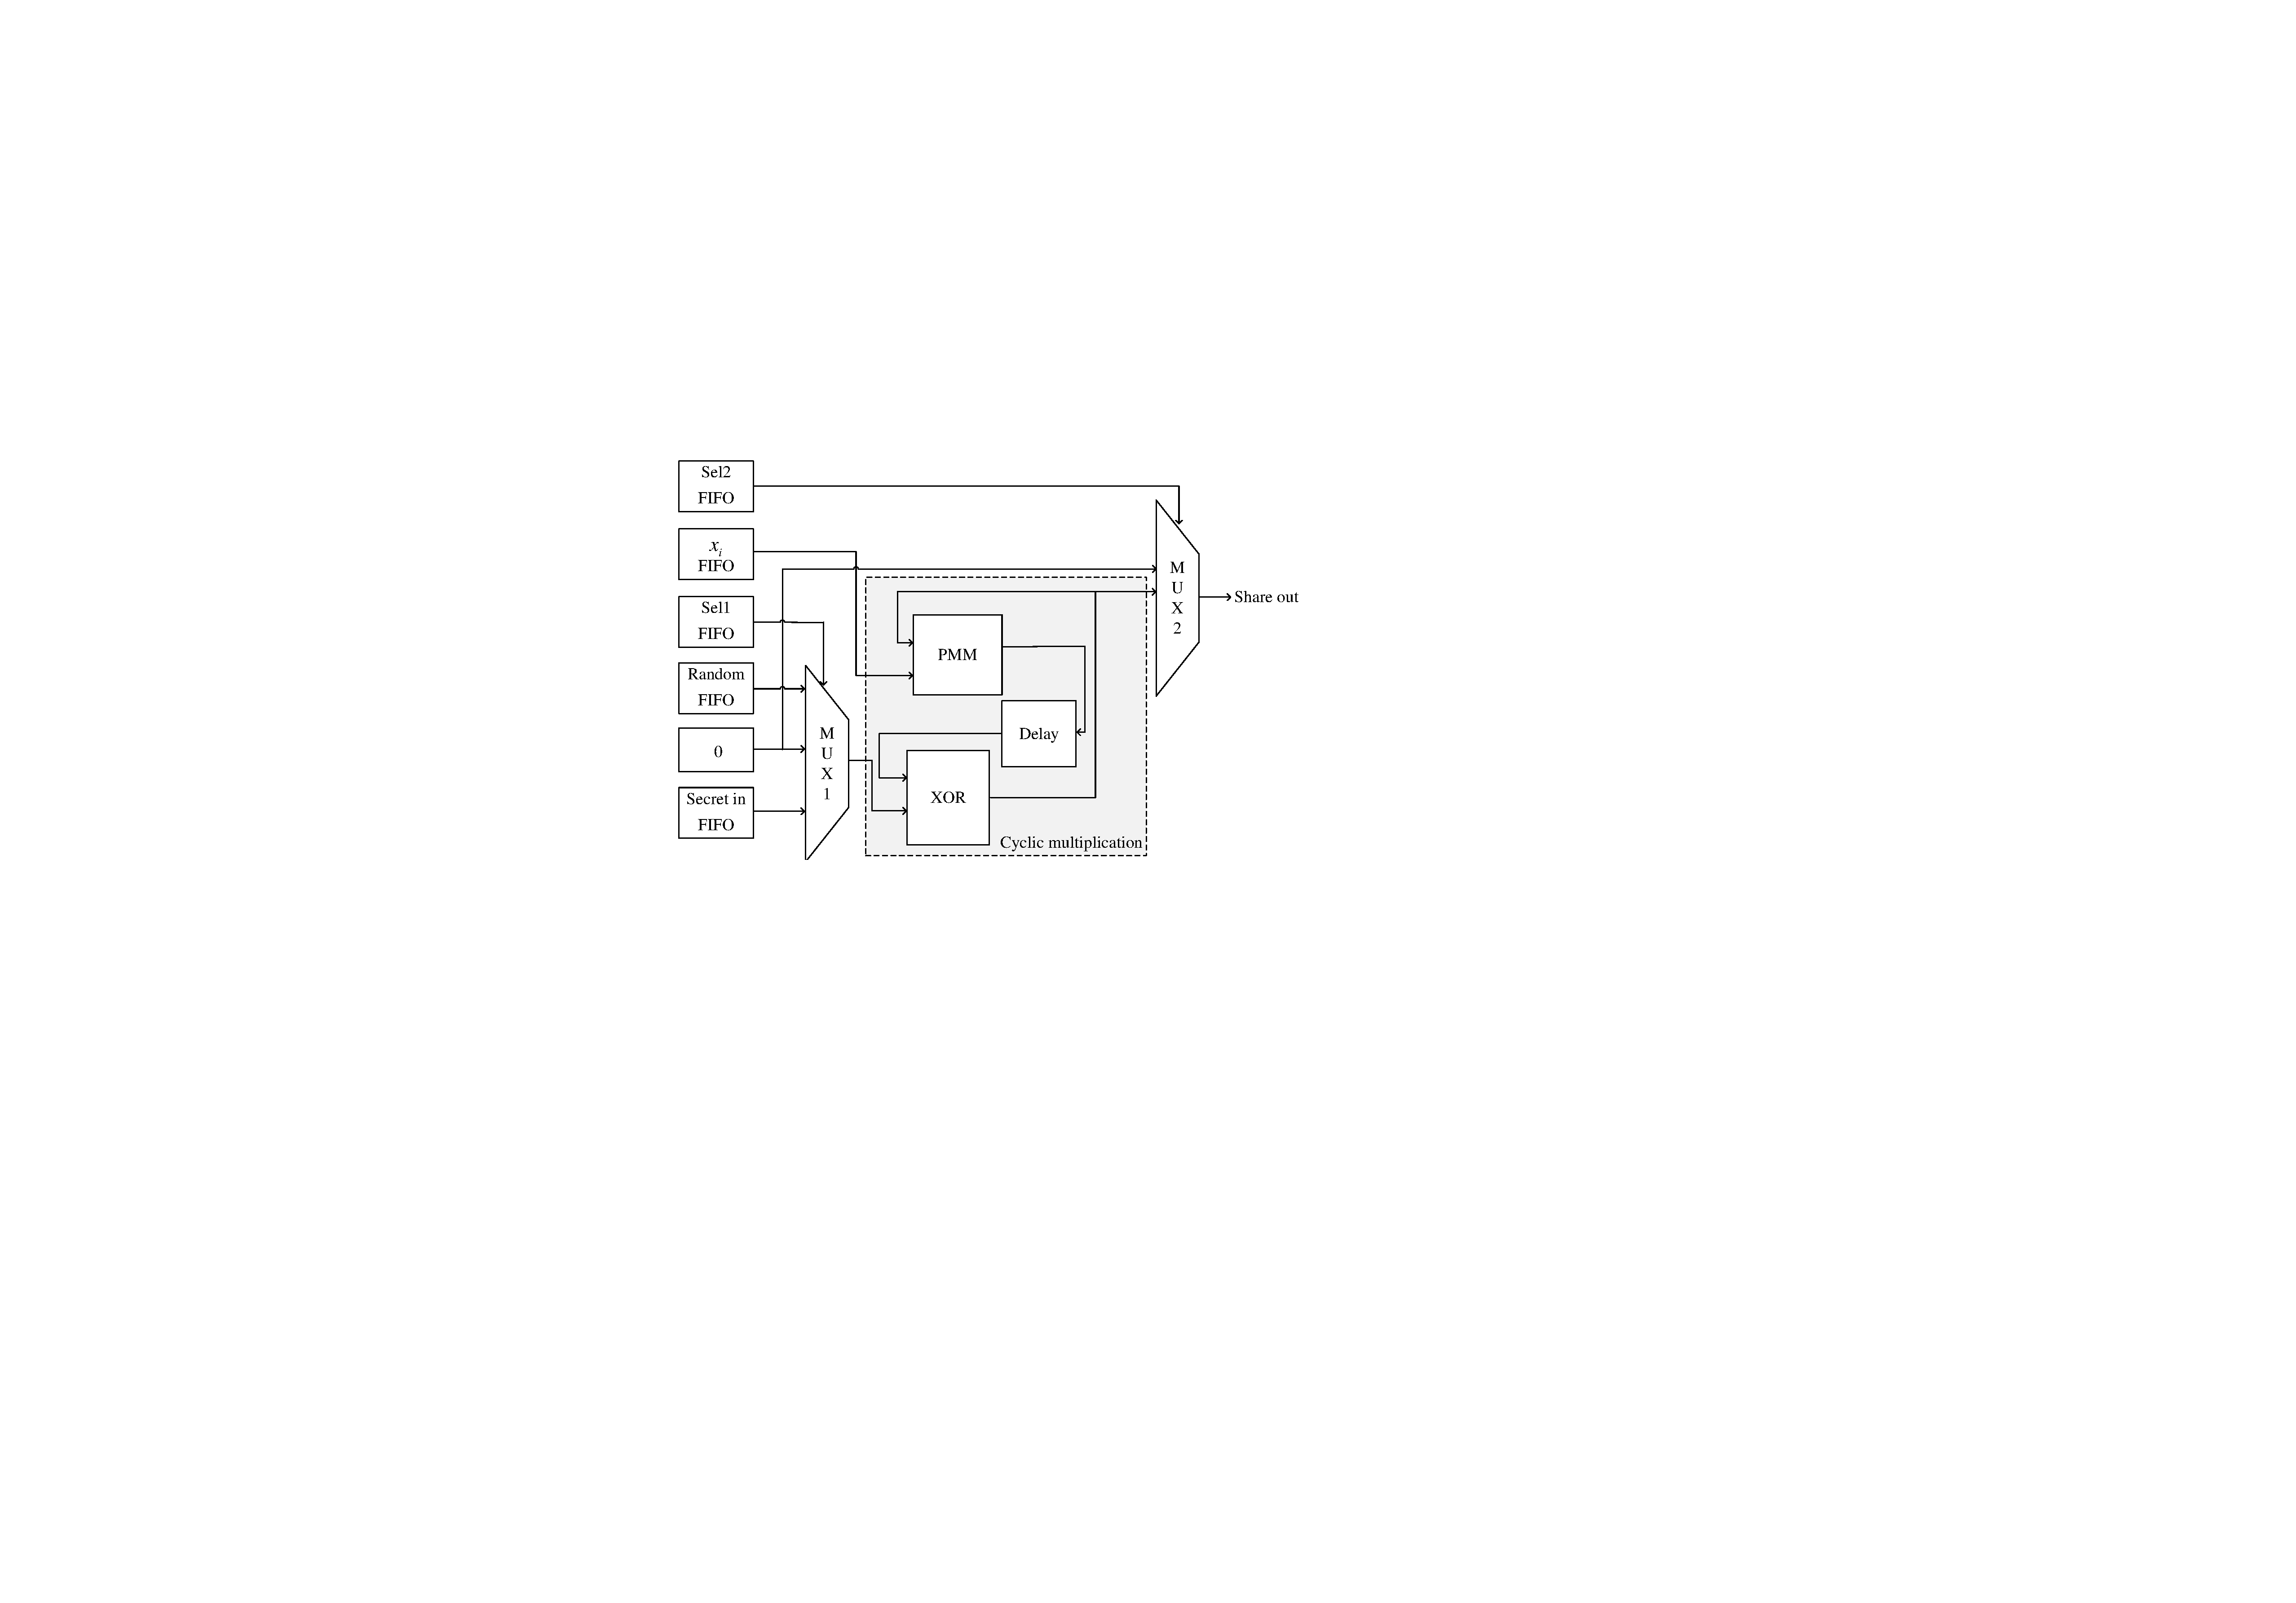
\includegraphics[width=8.5cm]{cyclic.eps}\\
		\caption{Optimized SGM}
		\label{fig06}
		\vspace{-2.0em}
	\end{center}
\end{figure}

In the SGM. The use of FIFO instead of ROM for data storage enables simultaneous reading and writing. In this way the large data of the 3D data cubes can be processed. The Sel1 FIFO controls MUX1 to pass in different data for calculation. A share generation requires 6 operations. As shown in Fig. \ref{fig07}.

The whole process consists of 6 operations:

\begin{enumerate}[(1)]
	\item Operation1: control MUX1 to pass in random number $a_2$ through Sel1 FIFO.
	\item Operation2: calculate $a_{2} \oplus 0$ in XOR while controlling $x_{i}$ FIFO pass in $x_{1}$.
	\item Operation3: calculate $a_{2}x_{1} $ in PMM while controlling MUX1 pass in $a_{1}$.
	\item Operation4: calculate $a_{1}\oplus a_{2} x_{1}$ in XOR while controlling $x_{i}$ FIFO pass in $x_{1}$.
	\item Operation5: calculate $a_{1}x_{1}  \oplus a_{2} x_{1}^{2}$ in PMM while controlling MUX1 pass in $a_{0}$.
	\item Operation6: calculate $a_{0}\oplus a_{1}x_{1}  \oplus a_{2} x_{1}^{2}$ in XOR while controlling the MUX2 enable side to pass out the final result.
\end{enumerate}

\begin{figure*}
	\begin{center}
		% Use the relevant command to insert your figure file.
		% For example, with the graphicx package use
		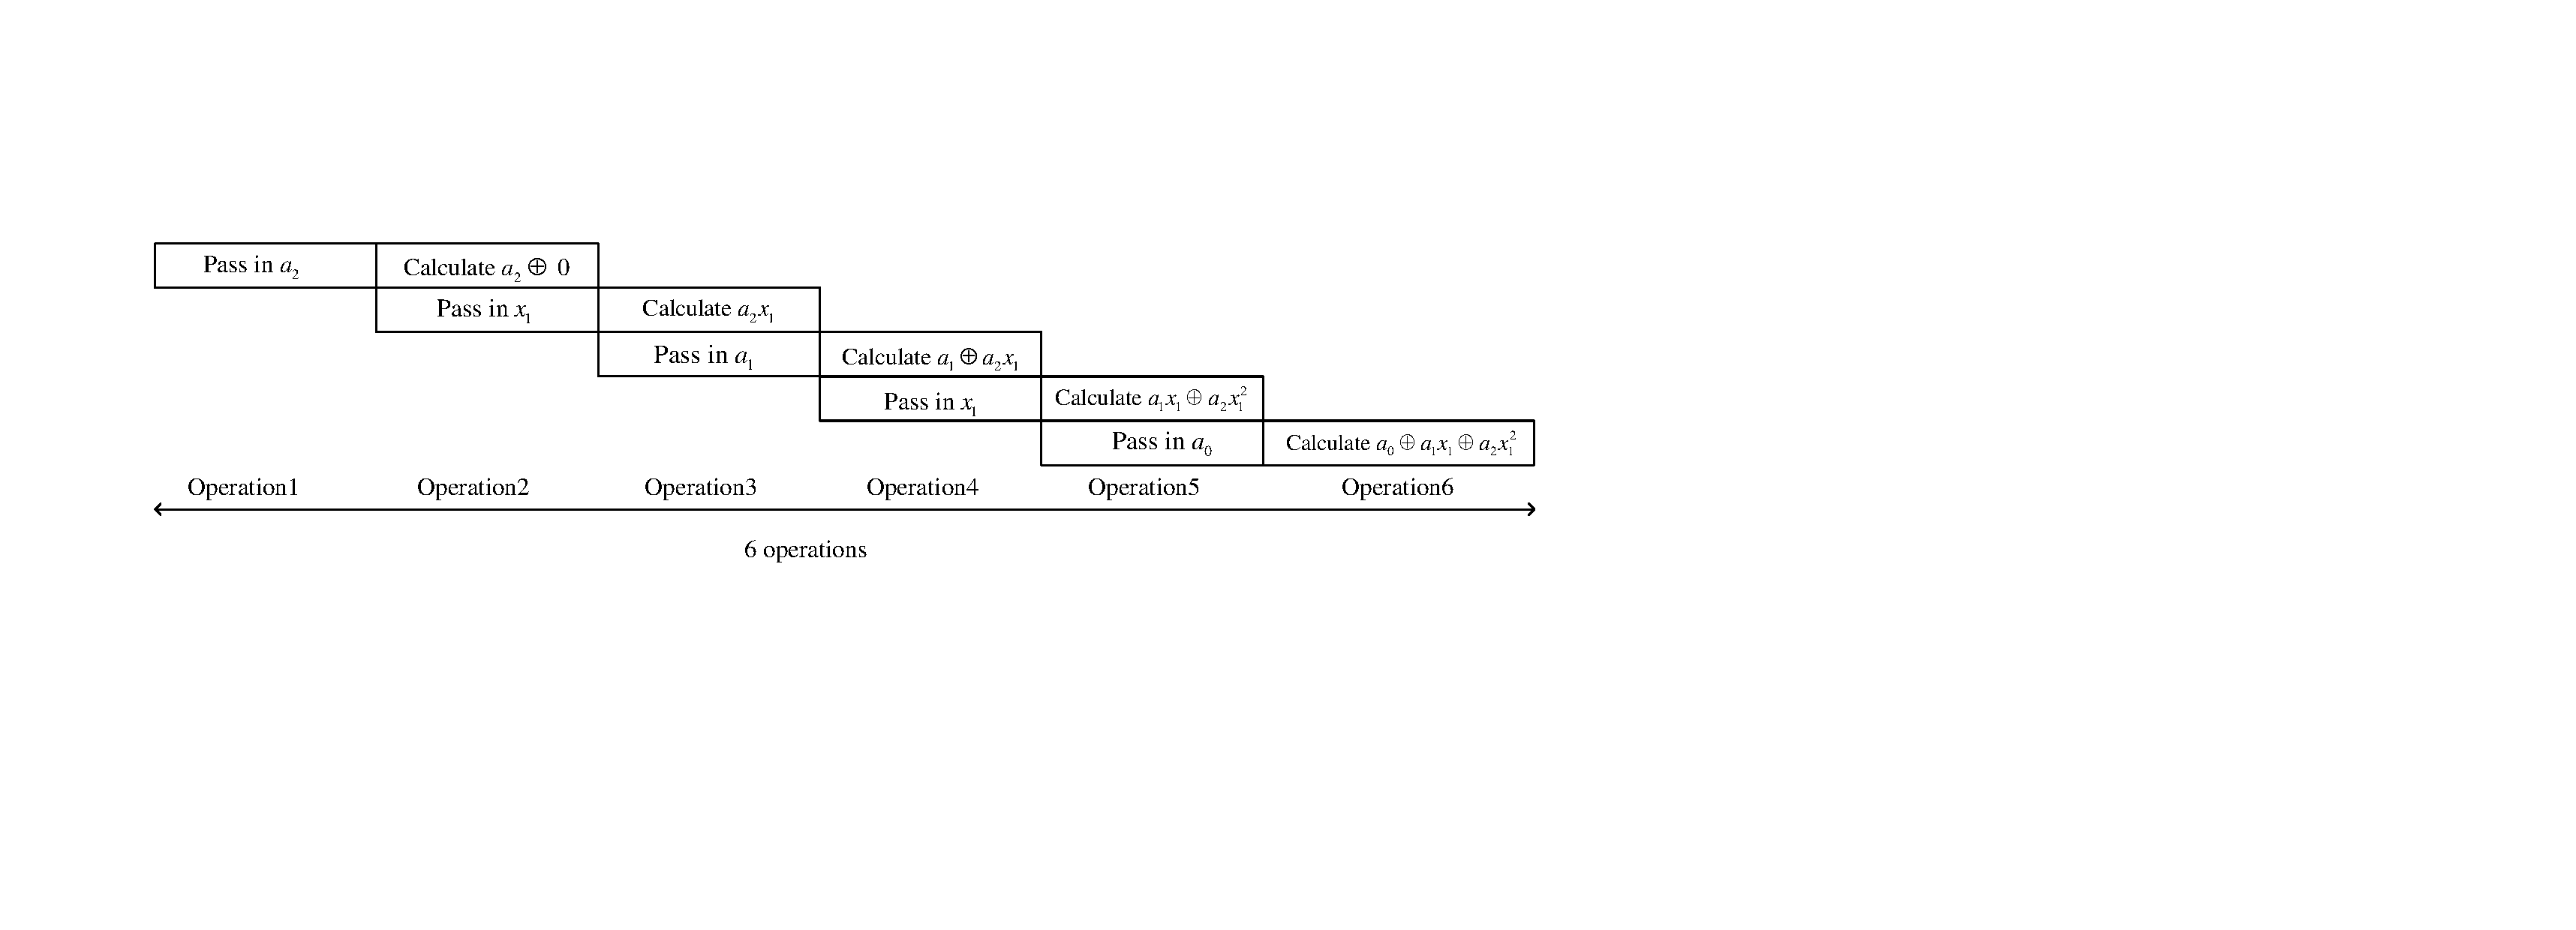
\includegraphics[width=0.85\textwidth]{cycle.eps}
		% figure caption is below the figure
		\caption{Loop pipelining}
		\label{fig07}       % Give a unique label\
		\vspace{-2.0em}
	\end{center}
\end{figure*}
It can be seen that a large amount of data is repeatedly passed into the PMM when sharing the 3D data cubes. To improve the speed of data sharing, the polynomial multiplication process therefore needs to be processed in parallel.

\subsubsection{Polynomial multiplication module}\label{subsec_NC-BPDVC_framework}

In the PMM. First, $X\times 0\mathrm{x} 01 \ldots X\times0\mathrm{x} 80$ should be calculated, and then the non-zero bits of $Y$ should be taken and multiplied with it separately. The two processing processes are carried out in parallel when designing the circuit. We divide it into $X$ processing and $Y$ processing. As shown in Fig. \ref{fig08} and Fig. \ref{fig09}.

\begin{figure}[!htb]
	\begin{center}
		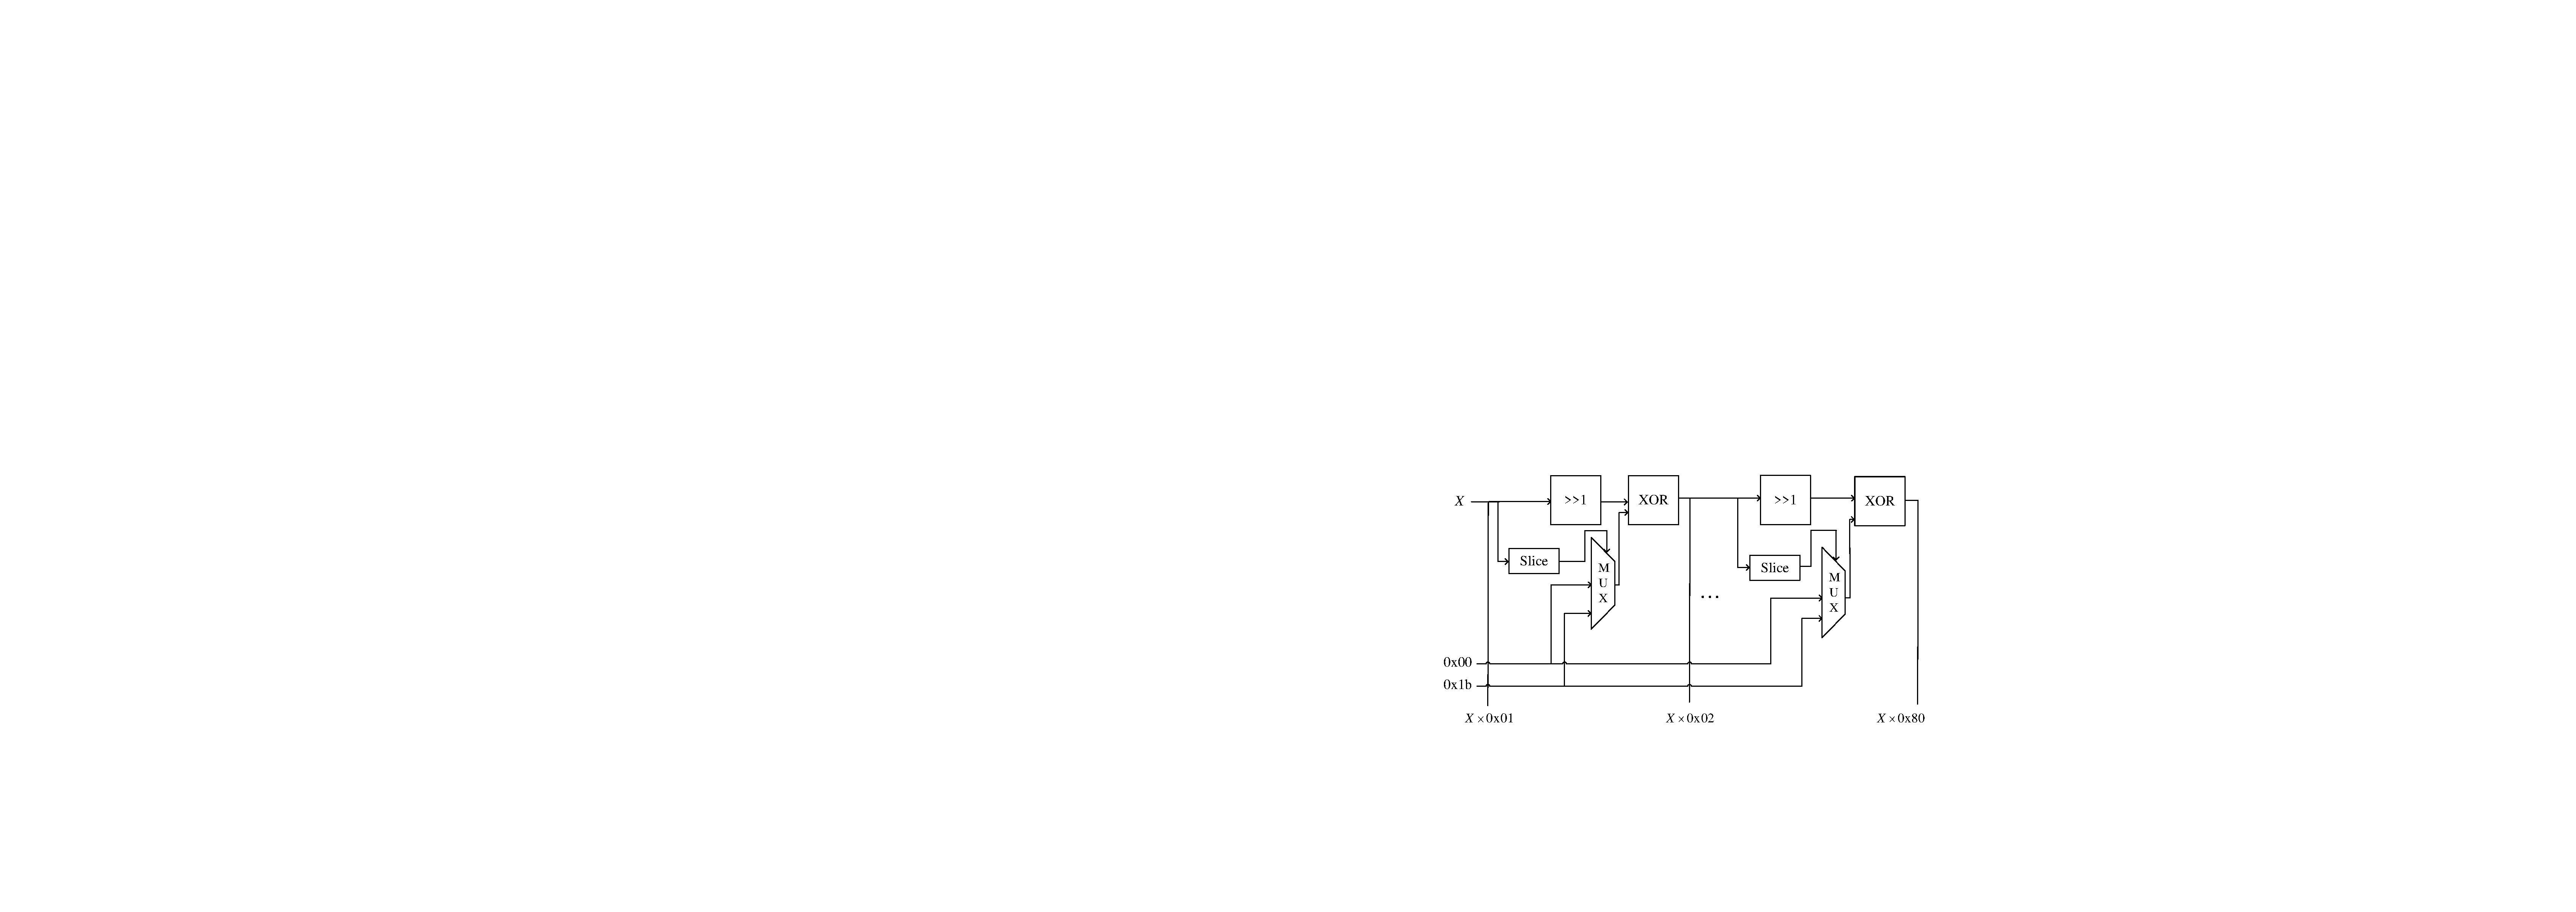
\includegraphics[width=8.5cm]{Mulin.eps}\\
		\caption{Polynomial multiplication $X$ processing}
		\label{fig08}
		\vspace{-1.0em}
	\end{center}
\end{figure}

After inputting $X$, shift $X$ one bit to the right and pass it to XOR. Extract the highest bit of $X$ by Slice to determine if there is a data overflow. If there is data overflow, then you need to control MUX input 0x1b to XOR.

While processing $X$, the other multiplier $Y$ is shifted one bit to the right. Then, the lowest bit of $Y$ is extracted and multiplied by the processed $X$. Finally, the results of all multiplications are passed into XOR. The result of multiplying $X$ and $Y$ is obtained.

\begin{figure}[!htb]
	\begin{center}
		\includegraphics[width=8.5cm]{Mulout.eps}\\
		\caption{Polynomial multiplication $Y$ processing}
		\label{fig09}
		\vspace{-2.0em}
	\end{center}
\end{figure}

\subsection{Secret reconstruction phase}\label{subsec_NC-BPDVC_framework}

In the secret reconstruction phase, the original secret data can be restored when $t$ or more shares are collected.

Shares are passed into the SRM (secret reconstruction module) in parallel for Lagrangian interpolation. As a result, the complete original secret is finally obtained. As shown in Fig. \ref{fig10}.

\begin{figure*}
	\begin{center}
		% Use the relevant command to insert your figure file.
		% For example, with the graphicx package use
		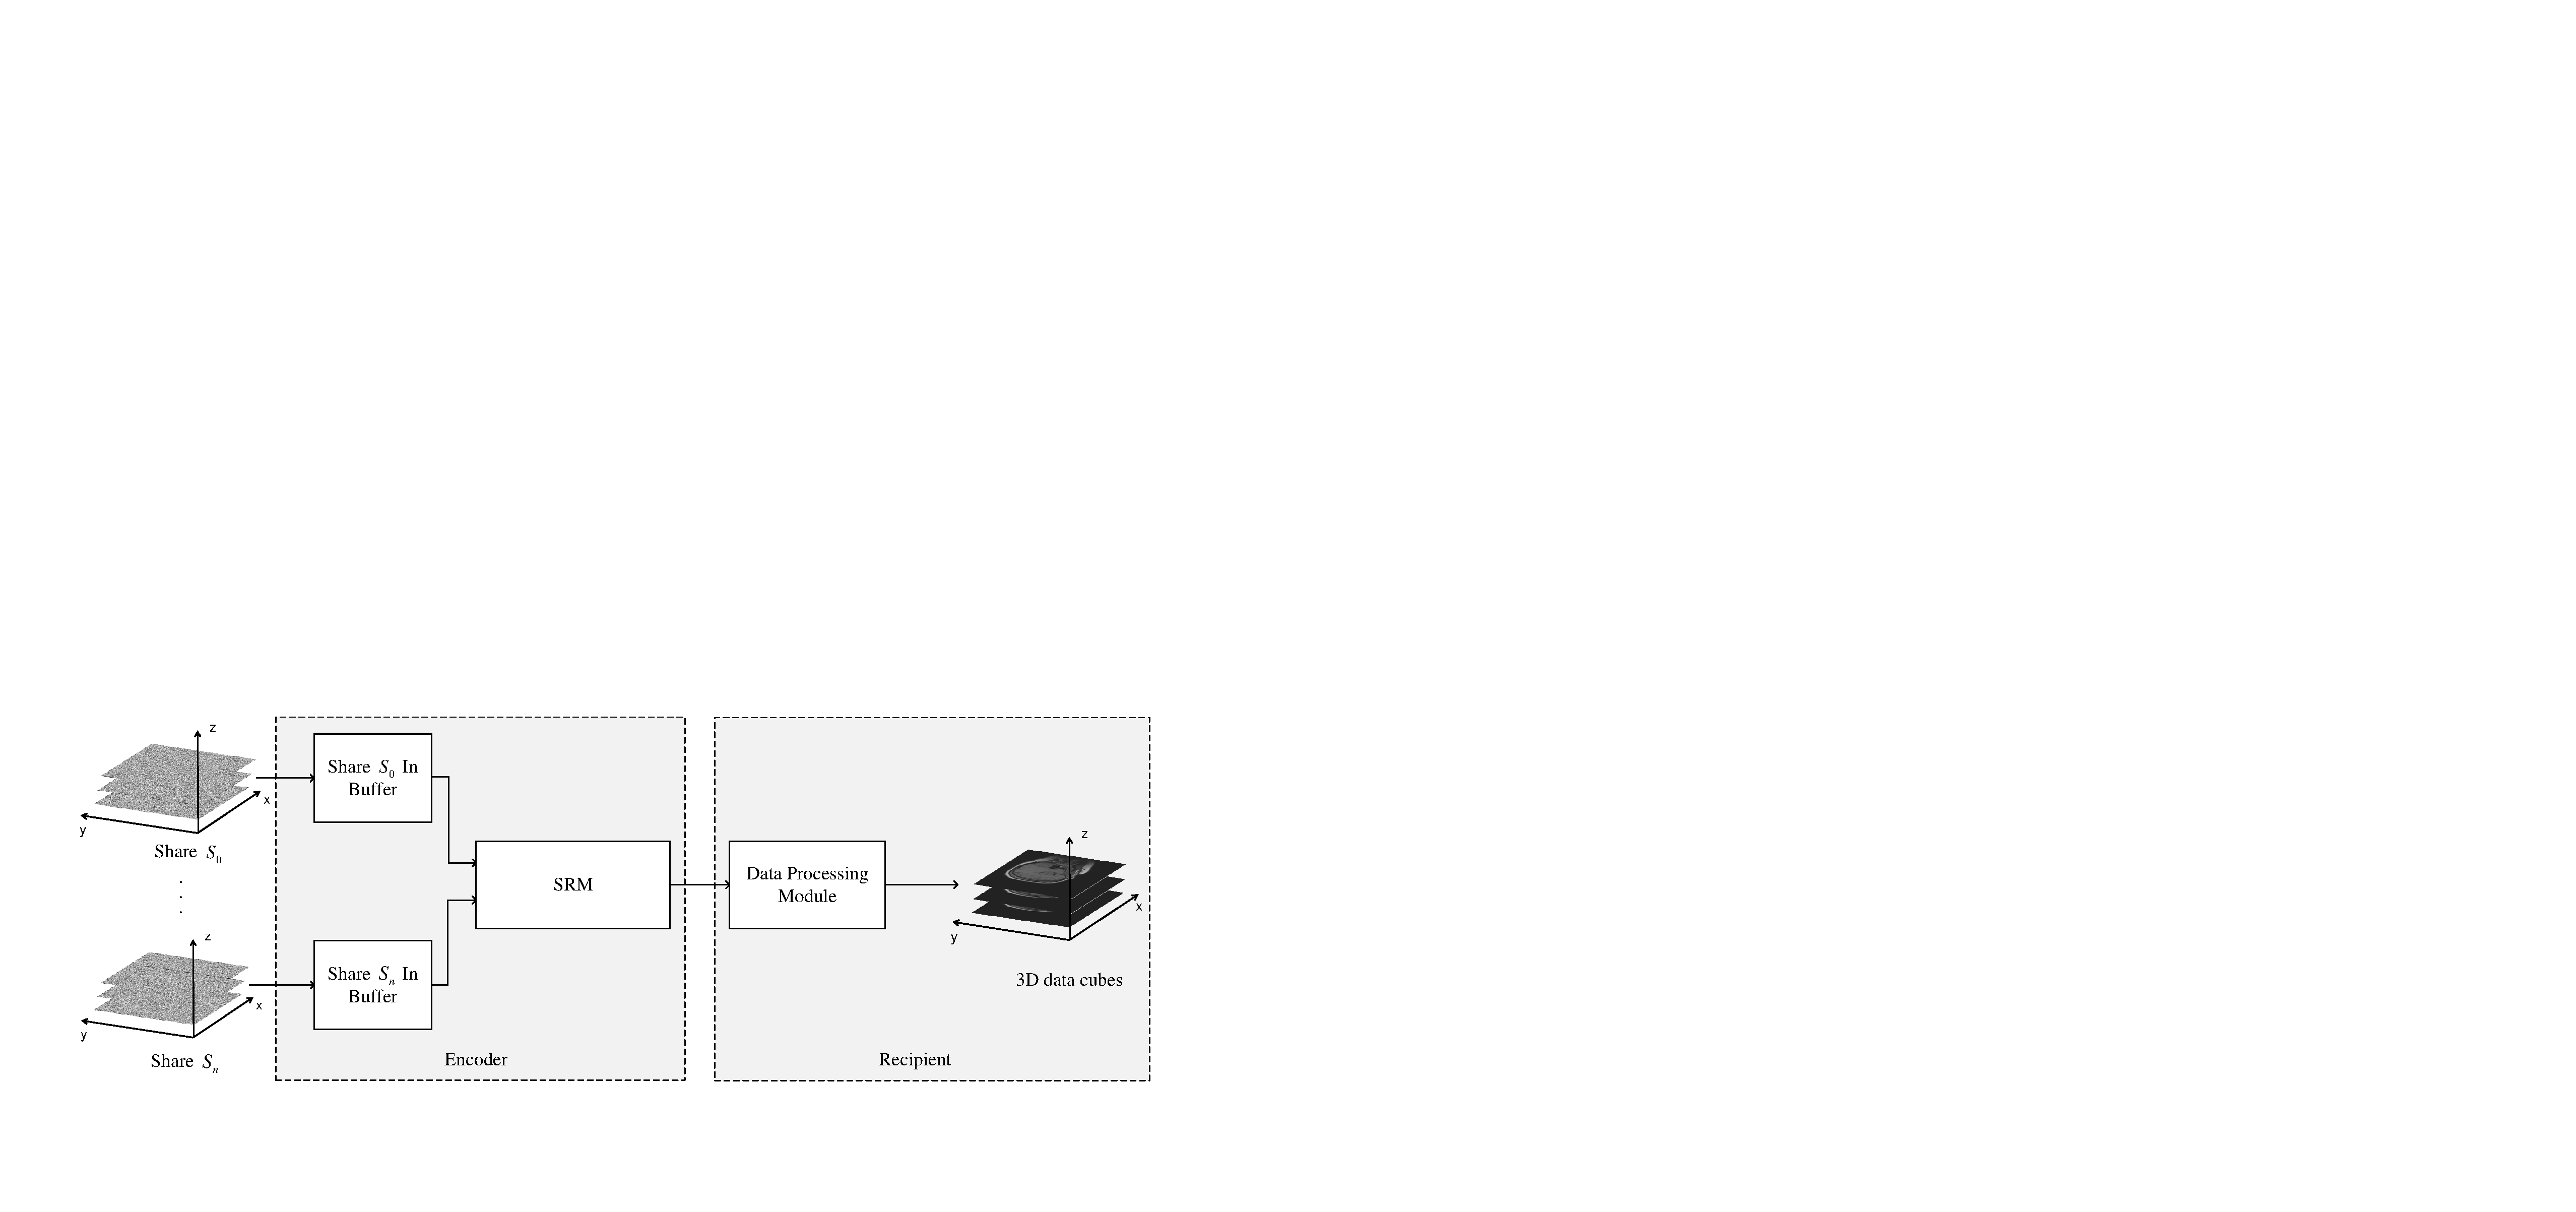
\includegraphics[width=0.85\textwidth]{SRM_jian.eps}
		% figure caption is below the figure
		\caption{{\color{red}Secret reconstruction phase}}
		\label{fig10}       % Give a unique label\
		\vspace{-2.0em}
	\end{center}
\end{figure*}
\subsubsection{Secret reconstruction module}\label{subsec_NC-BPDVC_framework}

Lagrangian interpolation method is used directly to perform the recovery. Taking (3,3)-threshold as an example, the polynomial of restoration can be expressed as

\begin{equation}
\begin{aligned}
a_{0}= & \frac{x_{2} \cdot x_{3}}{\left(x_{1}-x_{2}\right)\left(x_{1}-x_{3}\right)} f\left(x_{1}\right)+ \\
& \frac{x_{1} \cdot x_{3}}{\left(x_{2}-x_{1}\right)\left(x_{2}-x_{3}\right)} f\left(x_{2}\right)+ \\
& \frac{x_{1} \cdot x_{2}}{\left(x_{3}-x_{1}\right)\left(x_{3}-x_{2}\right)} f\left(x_{3}\right) \quad \bmod p(x).
\end{aligned}
\end{equation}

The coefficients of the Lagrangian interpolation method are fixed during the secret reconstruction. It can be calculated in advance and passed in through coefficient FIFO to save computation time.

As shown in Fig. \ref{fig11}, the shares and coefficients are passed simultaneously to the PMM through different FIFOs. The terms of the Lagrangian interpolation can be computed at the same time. Finally, the calculated terms are input to XOR to reconstruct the secret.

\begin{figure}[!htb]
	\begin{center}
		\includegraphics[width=8cm]{SRU.eps}\\
		\caption{Structure of the SRM}
		\label{fig11}
		\vspace{-2.0em}
	\end{center}
\end{figure}

The designed SGM and SRM can efficiently implement the secret sharing of 3D data cubes. They also have strong portability. They are also useful when conducting experiments related to secret sharing of 3D data cubes.

\section{Extensions to multi-party computation}\label{Sec_Multi-party}

Our proposed parallel circuits in the previous section can be extended to the four basic processes of multi-party computation, realizing efficient operations for multi-party computation. Section \ref{subsec41} describes how to perform operations on shares. Section \ref{subsec42} presents an example and analyzes it.

\subsection{Four basic processes of multi-party computation}\label{subsec41}
The essence of multi-party computation based on secret sharing is to perform computation on the generated shares. Since the share generation is linear, the reconstructed secret will perform the same computation. Depending on the object of the computation and the method of computation, the basic process of multi-party computation can be divided into additive process, multiplication process, double shares addition process and double shares multiplication process.


As shown in Fig. \ref{fig12}. If the user does not need to encrypt the calculation method, he can select the additive process and the multiplication process. If the user needs to encrypt the calculation method, he can select the double shares addition process and double shares multiplication process.

\begin{figure}[!htb]
	\begin{center}
		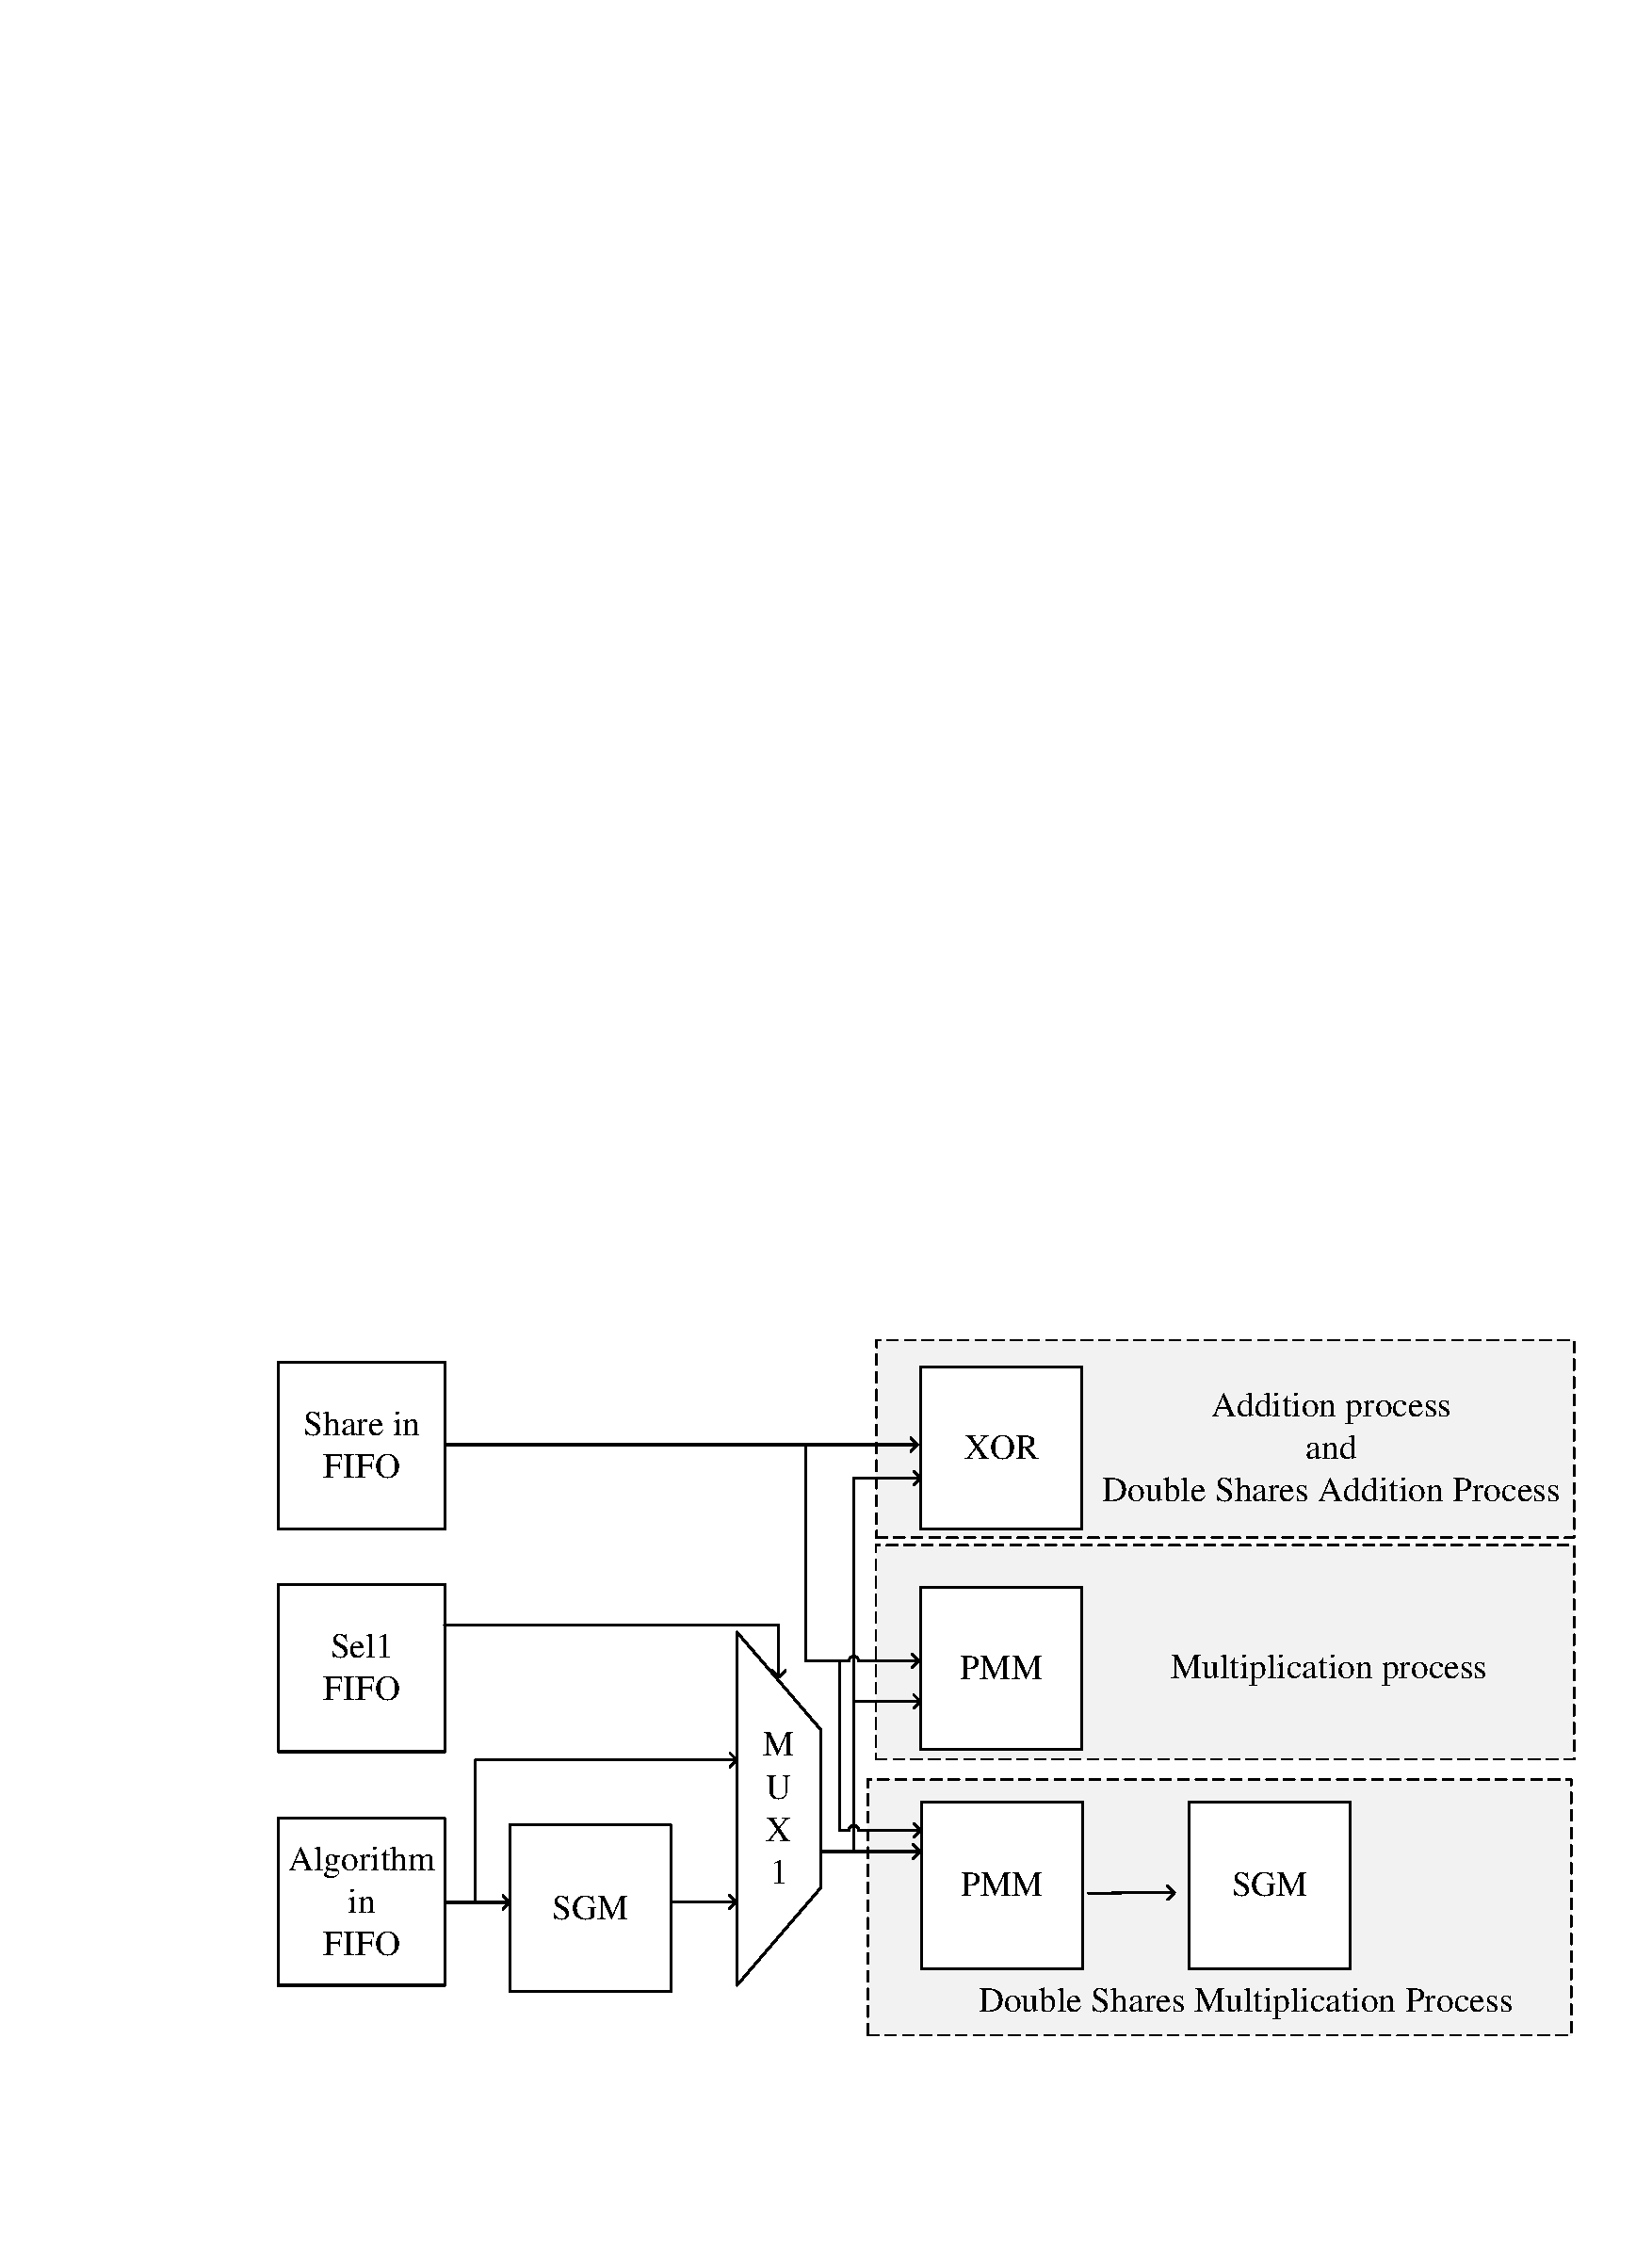
\includegraphics[width=8.5cm]{mulcom1.eps}\\
		\caption{Multi-party computation}
		\label{fig12}
		\vspace{-2.0em}
	\end{center}
\end{figure}

Algorithm in FIFO passes in the constants to perform operations on the shares. The Sel1 FIFO controls whether the output constants need to be generated as shares as well. The selected constants and shares are then passed into the computing system for operation.

The operations performed in the addition process and double shares addition process are XOR because addition and subtraction are replaced by XOR in the $GF (2^{8})$. The computed objects can all be shares or shares and constants.

The operations performed in the multiplication process is multiplication, {\color{red}which can be calculated directly using the ploynomial multiplication module.} The calculation is performed on shares and constants. The operation performed in the double shares multiplication process is multiplication. After multiplication, the double shares cannot be reconstructed, so a second sharing is required. The calculation is performed on both shares.

\subsection{An example of multi-party computation}\label{subsec42}

We pose a fundamental question to carry out an analysis of how our architecture accelerates multi-party computation.

Suppose Alice and Bob have value1 and value2 respectively. Mike needs to know the sum of value1 and value2, but Mike cannot know what value1 and value2 are.

\begin{figure*}[!htb]
	\begin{center}
		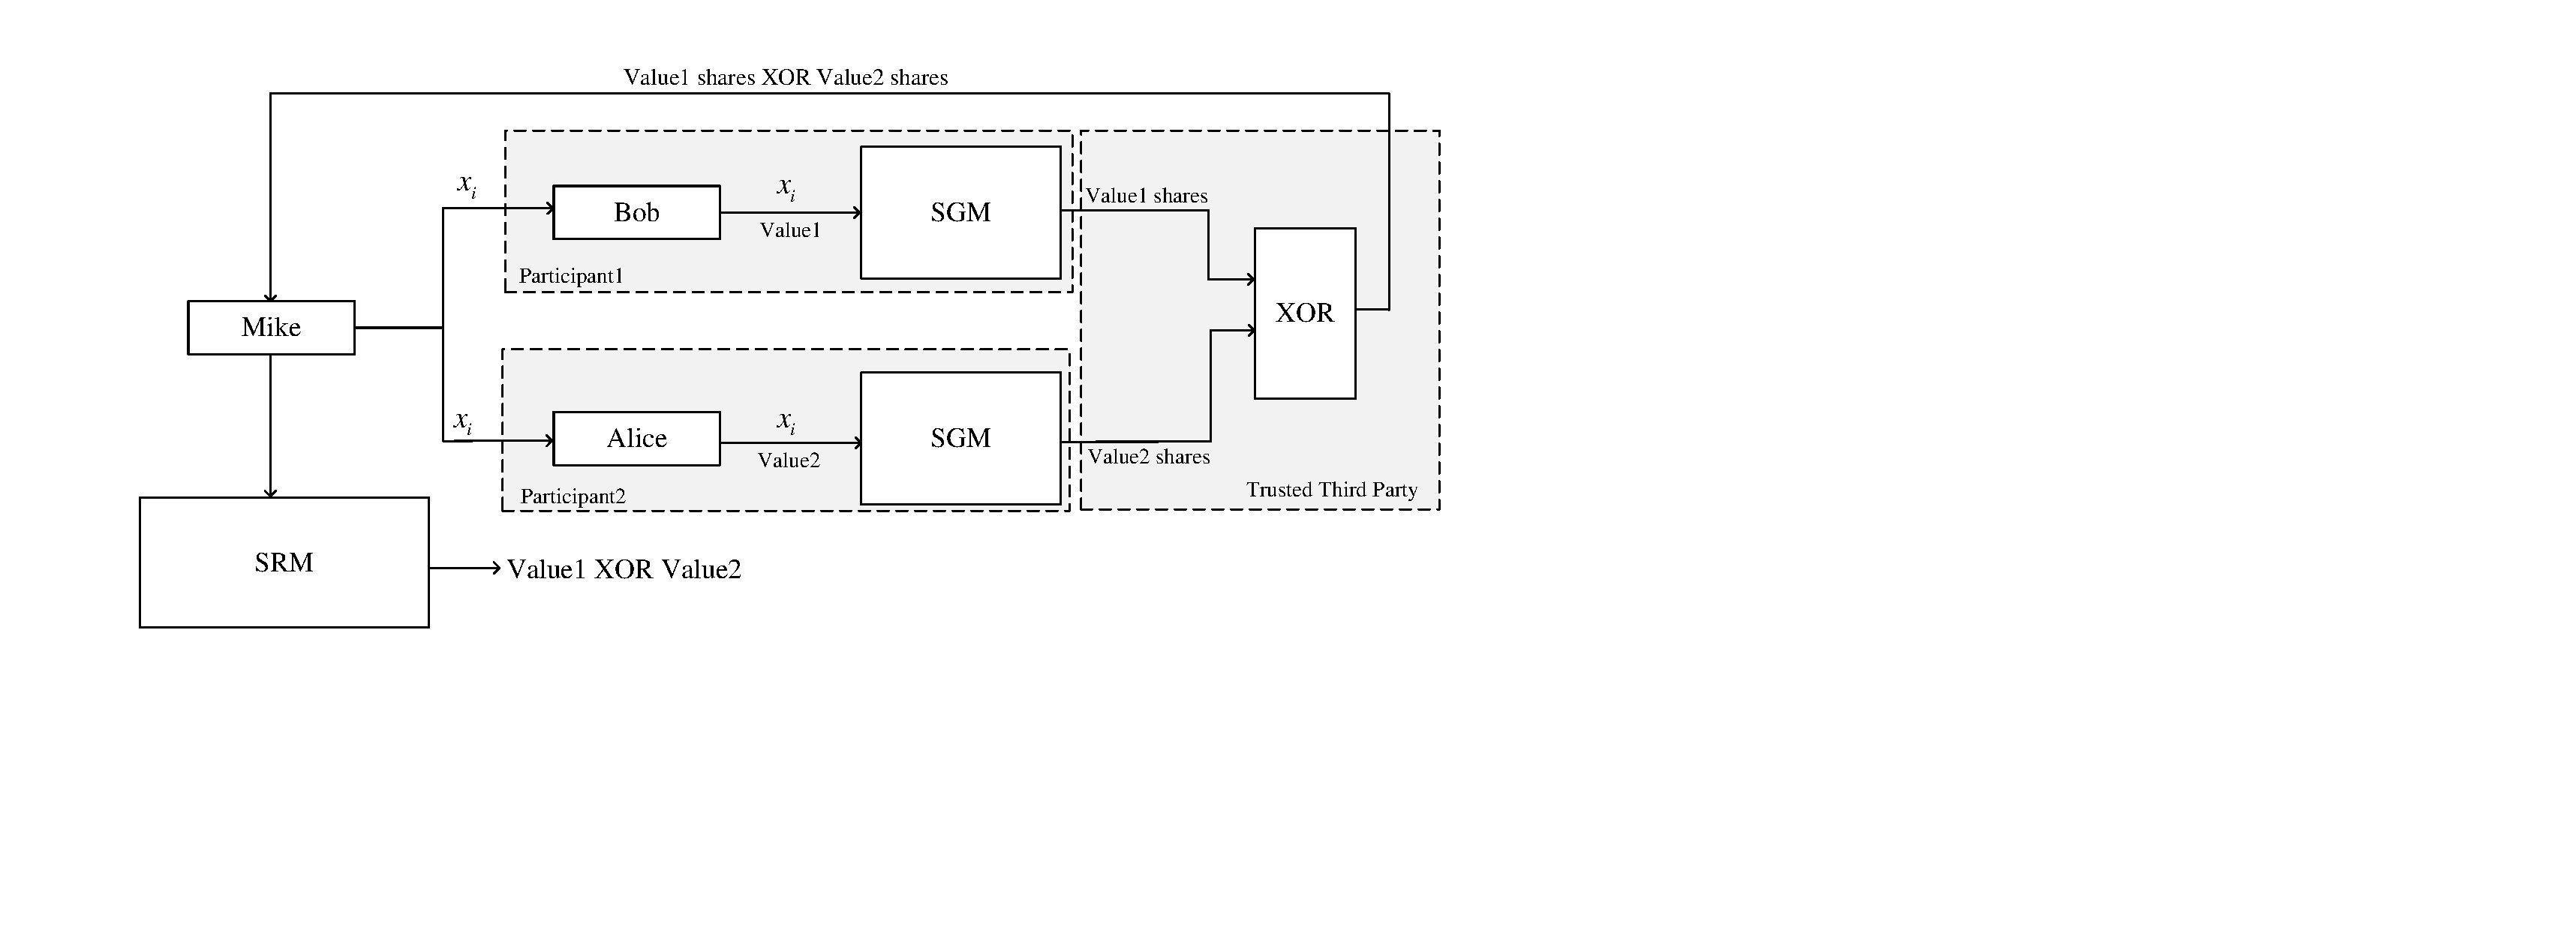
\includegraphics[width=12cm]{example.eps}\\
		\caption{An example of multi-party computation}
		\label{fig13}
		\vspace{-2.0em}
	\end{center}
\end{figure*}

In this process, the value needs to be shared in order not to leak information. So it is necessary to control MUX1 to select the value passed in after sharing.

As shown in Fig. \ref{fig13}. First, Mike needs to pass the $x_{i}$ to Bob and Alice. Bob and Alice pass their value into the SGM to generate the value shares based on the obtained $x_{i}$. The value shares are then passed to a trusted third party for computing. After the operation, the value1 shares XOR value2 shares are obtained and passed back to Mike. Finally, Mike passes the received values into the SRM to get value1 XOR value2. 

For Bob and Alice, what they pass to the third party is the value after sharing. The third party does not know $x_{i}$ so it cannot reconstruct value1 and value2. Bob and Alice's values are secure. {\color{red}Mike can only get value1 XOR value2 after performing the reconstruction, so the values of Bob and Alice will not be leaked during the reconstruction process either.}

If the algorithm needs to perform multiple operations, multiple secret sharing and secret reconstruction are required. If the amount value is large, such as a 3D data cubes. Serial computation will be very time-consuming compared to parallel. Using our designed structure we can accelerate the process in parallel so that the process can be implemented quickly.

\section{Experimental results and discussions}\label{Sec_experiments}

In this section, we use the constructed FPGA system to carry out the secret sharing process of the 3D data cubes. Section \ref{subsec51} focuses on the correctness and privacy. The recoverability of the secret images is analyzed by conducting recovery experiments on different numbers of shares. Section \ref{subsec52} analyzes the consumption of circuit resources. Section \ref{subsec53} focuses on the time complexity. We have made a comparison between serial and parallel runtimes.

We choose different 3D data cubes for the experiments to ensure the accuracy and reliability of the experimental results. In this section, 01-head is used as an example for analysis. Its 3D diagram is drawn with 3D slicer as shown in Fig. \ref{fig14}.

\begin{figure}[!htb]
	\begin{center}
		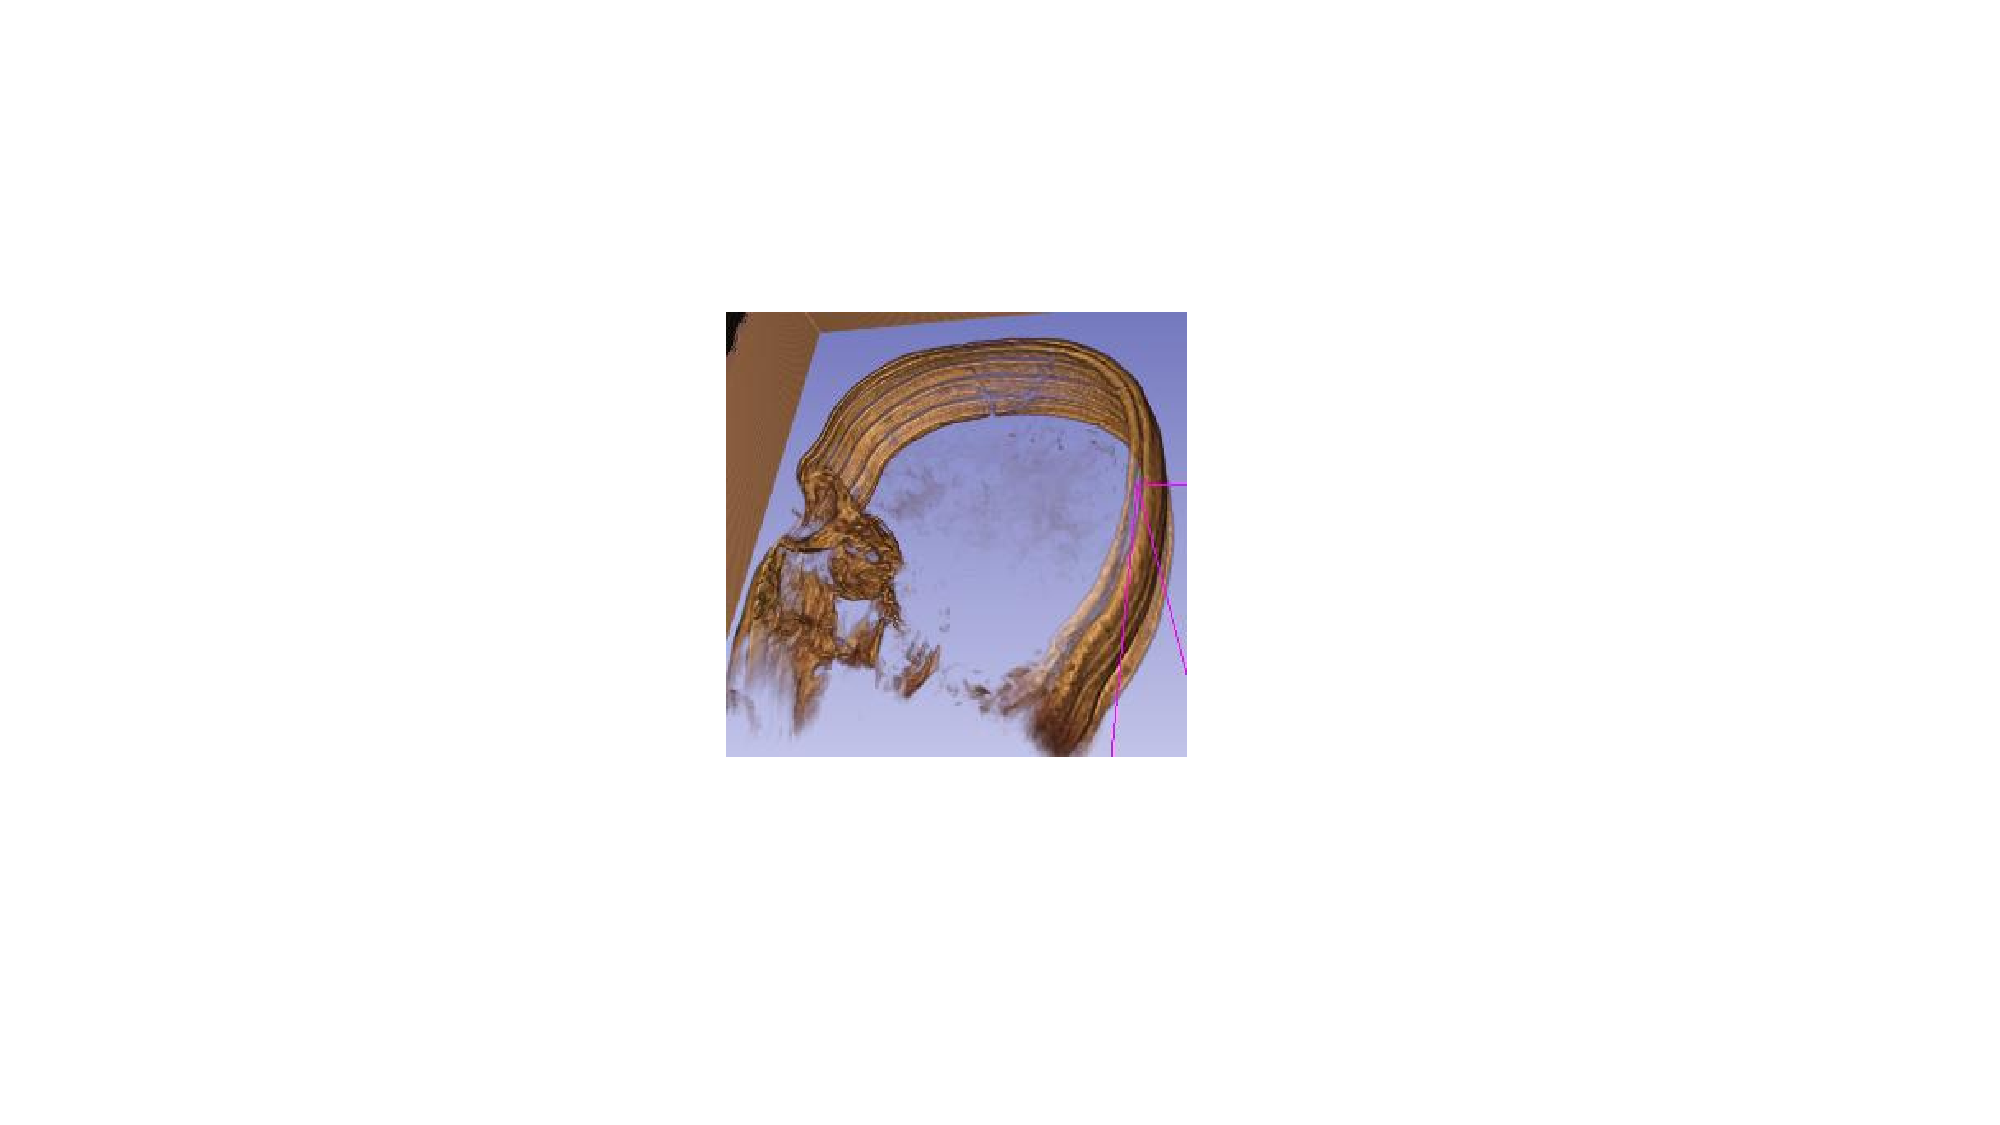
\includegraphics[width=3cm]{01-head.eps}\\
		\caption{01-head 3D diagram}
		\label{fig14}
		\vspace{-1.0em}
	\end{center}
\end{figure}

\subsection{Correctness and privacy}\label{subsec51}

\subsubsection{Recoverability of different numbers of shares}\label{subsec_Encoding}

The 3D data cubes can be sliced to get more details for analysis, and it is also a common way to process the 3D data cubes. Since the 3D data cubes have three dimensions, we choose three different slicing directions. These are shown in Fig. \ref{fig15}.

\begin{figure}[h]
	\begin{center}
		\includegraphics[width=8.5cm]{slice_dir.eps}\\
		\caption{Slices in three different directions}
		\label{fig15}
		\vspace{-2.0em}
	\end{center}
\end{figure}

The (3, 4)-threshold is chosen as an example. We use different numbers of shares for secret reconstruction to detect recoverability. The slice with the position in the middle is selected for display. The obtained results are shown in Fig. \ref{fig16}.

\begin{figure*}
	\centering
	\subfigure[Recoverability of four shares]{
		\begin{minipage}[t]{0.5\linewidth}
			\centering
			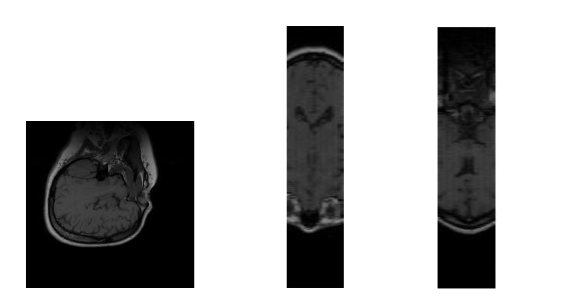
\includegraphics[width=2.6in]{4-1.eps}\\
		\end{minipage}%
	}%
	\subfigure[Recoverability of three shares]{
	\begin{minipage}[t]{0.5\linewidth}
		\centering
		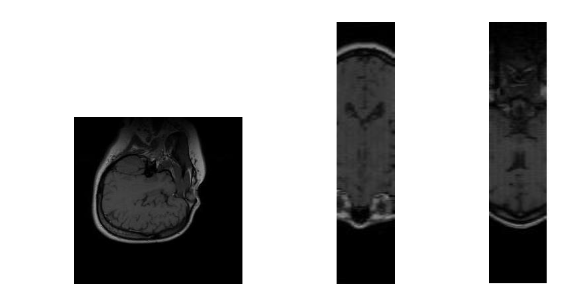
\includegraphics[width=2.6in]{3-1.eps}\\
	\end{minipage}%
	}%

\subfigure[Recoverability of two shares]{
	\begin{minipage}[t]{0.5\linewidth}
		\centering
		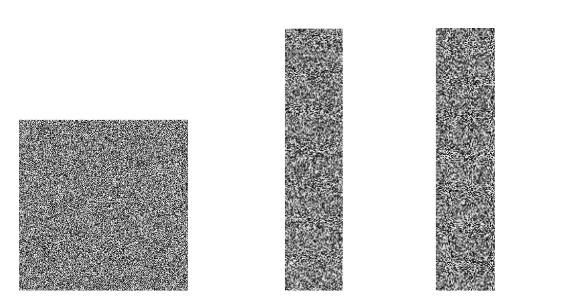
\includegraphics[width=2.6in]{2-1.eps}\\
	\end{minipage}%
}%
\subfigure[Recoverability of one share]{
	\begin{minipage}[t]{0.5\linewidth}
		\centering
		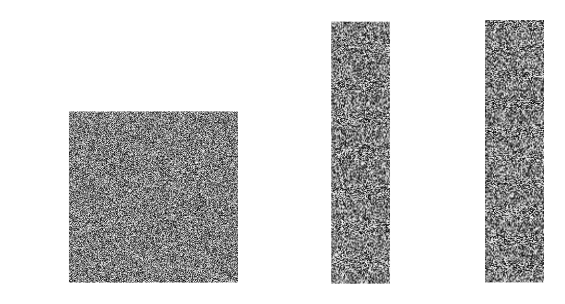
\includegraphics[width=2.6in]{1-1.eps}\\
	\end{minipage}%
}%
	\centering
	\caption{The central slice of the secret image recovered from different number of shares}
	\vspace{-0.2cm}
	\label{fig16}
\end{figure*}

We can get it by experiment. {\color{red}When the number of shares is less than 3, the polynomial used to reconstruct the secret will have one item missing. So the Lagrangian interpolation method will not be able to restore the secret.} When the number of shares is greater than or equal to 3, the secret image can be recovered. The result is in accordance with the threshold we set.

\subsubsection{Entropy calculation for shares}\label{subsec_Encoding}

The histogram of an image gives distribution of each value in an image. A natural image usually has a screwed histogram while an encrypted or scrambled image has a flat histogram. So we use histogram of the share to characterize the randomness on share. Fig. \ref{fig17(a)} shows the histogram of the original secret image. The histograms of two shares are shown in Fig. \ref{fig17(b)} and Fig. \ref{fig17(c)}, respectively. 

As shown in Fig. \ref{fig17}. The histogram of the image before encryption is mainly concentrated around pixel value 20. The pixels of the encrypted image are evenly distributed between 0 and 255. This indicates that the security of the image can be ensured by this scheme.

\begin{figure}[!htb]
	\centering
	\subfigure[\label{fig17(a)}]{
		\begin{minipage}[t]{0.5\linewidth}
			\centering
			\includegraphics[width=1.5in]{fanga.eps}
		\end{minipage}
	}%
	\subfigure[\label{fig17(b)}]{
		\begin{minipage}[t]{0.5\linewidth}
			\centering
			\includegraphics[width=1.5in]{fangb.eps}
		\end{minipage}
	}%

	\subfigure[\label{fig17(c)}]{
		\begin{minipage}[t]{0.5\linewidth}
			\centering
			\includegraphics[width=1.5in]{fangc.eps}
		\end{minipage}
	}%
	\centering
	\caption{Original image histogram and share histogram: (a)Secret image pixel histogram. (b)Histogram of share when $x_{i}$=2. (c) Histogram of share when $x_{i}$=4.}
	\label{fig17}
\end{figure}

Entropy in information theory was proposed by Shannon. It can be used to express the degree of redundancy of information.

A signal or source having uniform distribution corresponds to large entropy. So we can use entropy to characterize the randomness of a share image. The entropy can be calculated as

\begin{equation}
H(x_{i})=-\sum_{i=1}^{n} p\left(x_{i}\right) \log p\left(x_{i}\right),
\end{equation}where $n$ represents the possible values of the random variable, $x_{i}$ represents the random variable, and $p\left ( x_{i} \right ) $ represents the probability function of $x_{i}$.

As shown in Table \ref{tab1}, the entropy value of the image after sharing is greater compared to the secret image. It means that after the designed system is processed, it has more information security.

\begin{table*}[!htb]
	\begin{center}
	\caption{Entropy of the histogram}\label{tab1}%
	\begin{tabular}{ccccc}
		\toprule
		Secret Image&Share at&Share image at&Share at&Share at\\
		&$x_{i}$=2&$x_{i}$=4&$x_{i}$=6&$x_{i}$=8\\
		\midrule
		1.5149&5.1955&5.1949&5.1948&5.1940\\
		\bottomrule
	\end{tabular}
	\end{center}
\end{table*}

\subsection{Circuit resource consumption analysis}\label{subsec52}

The circuit resource consumption of FPGA is an important metric for evaluating circuit performance. In this section, a comparison is made between the circuit resource utilization for parallel operation and serial operation. {\color{red}Since the selected comparison scheme is implemented in software and the implementation is serial. In order to be able to compare parallel and serial at the same level, we built circuits for comparison according to the operational characteristics of parallel and serial. Serial can generate only one share at the same time and parallel can generate four shares at the same time. So the parallel implementation requires more circuit resources.}

\begin{table*}[!htb]
	\begin{center}
	\caption{{\color{red}Circuit resource consumption}}\label{tab2}
	\setlength{\tabcolsep}{6mm}{
	\renewcommand{\arraystretch}{1.3}
\begin{tabular}{c|cc|cc}
	\hline
	\multirow{2}{*}{(3, 4)-threshold} & \multicolumn{2}{c|}{Serial}        & \multicolumn{2}{c}{Parallel}          \\ \cline{2-5} 
	& \multicolumn{1}{c|}{Yan's\cite{xing2022information}} &Qin's\cite{qin2021reversible} & \multicolumn{1}{c|}{Optimized circuit} & Unoptimized circuit \\ \hline
	LUT                & 56                     & 3053 & 5018                    & 3270 \\
	FF                 & 88                     & 6832 & 11077                   & 7409 \\
	DSP                & 6                      & 80   & 105                     & 72   \\ \hline
\end{tabular}}
\vspace{-2.0em}
	\end{center}
\end{table*}

In Table \ref{tab2}, polynomial calculation consumes more circuit resources than normal calculation. In the case of both using polynomial calculation, the serial operation uses 85 DSP (digital signal processing), while the parallel operation uses 105 DSP. The number of LUT (lookup table) is reduced by $35\%$, the number of FF (flip flop) by $33\%$, and the number of DSP by $32\%$ after optimization. The optimized circuit has improved the utilization of FF, LUT and DSP.

\subsection{Time complexity analysis}\label{subsec53}

In this section, our scheme is compared with Yan's and Qin's. Yan's and Qin's schemes run serially while our scheme runs in parallel. There are two main aspects. Section \ref{subsec531} is the theoretical analysis, including time complexity and circuit delay. Section \ref{subsec532} is the actual running time.

\subsubsection{Time complexity and circuit delay}\label{subsec531}

The time complexity refers to the number of basic operations in the algorithm, denoted by $n$ as $O(n)$.

\begin{table}[!htb]
	\caption{Computational complexity comparison}\label{tab3}
	\label{1111}    
	\begin{tabular}{cc}
		\toprule
		(3, 4)-threshold&Algorithm complexity\\
		\midrule
		Yan’s\cite{xing2022information}&$O(n^{3} )$\\
		Qin‘s\cite{qin2021reversible}&$O(n^{4} )$\\
		Our&$O(n^{2} )$\\
		\bottomrule
	\end{tabular}
\end{table}

Parallel operations use fewer loop structures. As can be seen from Table \ref{tab3}, the time complexity of secret sharing through parallel operations is lower compared to serial operations.

The most significant factor affecting parallel circuits is the circuit delay. It represents the efficiency of the circuit in processing data. So we mainly make a comparison between the circuit delay of serial and parallel processing.

Since the simulation is performed on the system generator, the delay of each device is set based on the base settings of the system generator.

\begin{table*}[!htb]
	\begin{center}
	\caption{Circuit delays for different schemes}\label{tab4}
	\begin{tabular}{ccccc}
		\toprule
		(3, 4)-threshold&PMM delay&SGM delay&SRM delay&Total delay of the circuit\\
		\midrule
		Yan’s\cite{xing2022information}&0&44&50&94\\
		Qin‘s\cite{qin2021reversible}&79&956&239&1274\\
		Our&18&37&55&110\\
		\bottomrule
	\end{tabular}
	\end{center}
\end{table*}

\begin{table*}[!htb]
		\begin{center}
	\caption{Total circuit delay for different schemes}\label{tab5}
	\label{1111}    
	\begin{tabular}{cccc}
		\toprule
		(3, 4)-threshold&Polynomial calculation&Full restoration&Total delay\\
		\midrule
		Yan’s\cite{xing2022information}&No&No&$94 \times$ Total number of pixels\\
		Qin‘s\cite{qin2021reversible}&Yes&Yes&$1274\times$ Total number of pixels\\
		Our&Yes&Yes&$110+$  Total number of pixels\\
		\bottomrule
	\end{tabular}
	\end{center}
\end{table*}

From Table \ref{tab4} and \ref{tab5}, we can get that our scheme has less circuit delay than Qin's and more than Yan's. This is because the polynomial calculation is more complex, so more circuit structures are required.

As can be seen from the total delay, multiple data can be processed simultaneously during parallel operation. Parallel operation is much more efficient than serial operation when dealing with 3D data cubes.

\subsubsection{Actual running time}\label{subsec532}

The actual running time is tested by conducting experiments on different 3D data cubes. The experimental results of some of the 3D data cubes are given as shown in Table \ref{tab6}. As the amount of data in the 3D data cubes becomes larger, the processing efficiency of our solution becomes more and more efficient. The rest of the experimental results are placed on Github.
\url{https://github.com/1184745459/3D-data-cubes-experimental-results} 

\begin{table*}[!htb]
\begin{center}
	\caption{Actual time spent in the experiment}\label{tab6}
	\label{11111}    
	\begin{tabular}{ccccc}
		\toprule
		(3, 4)-threshold&Number of data&Yan’s\cite{xing2022information}&Qin‘s\cite{qin2021reversible}&Our\\
		\midrule
		01-head&3801088&3h12min&6h34min&30min\\
		03-CT-carotid&5023272&4h11min&8h40min&38min\\
		04-skull&13303808&11h12min&22h59min&1h45min\\
		05-cube1&16711680&14h4min&28h52min&2h11min\\
		\bottomrule
	\end{tabular}
	\end{center}
\end{table*}

\begin{figure}[!htb]
	\centering
	\subfigure[\label{fig18(a)}]{
		\begin{minipage}[t]{0.5\linewidth}
			\centering
			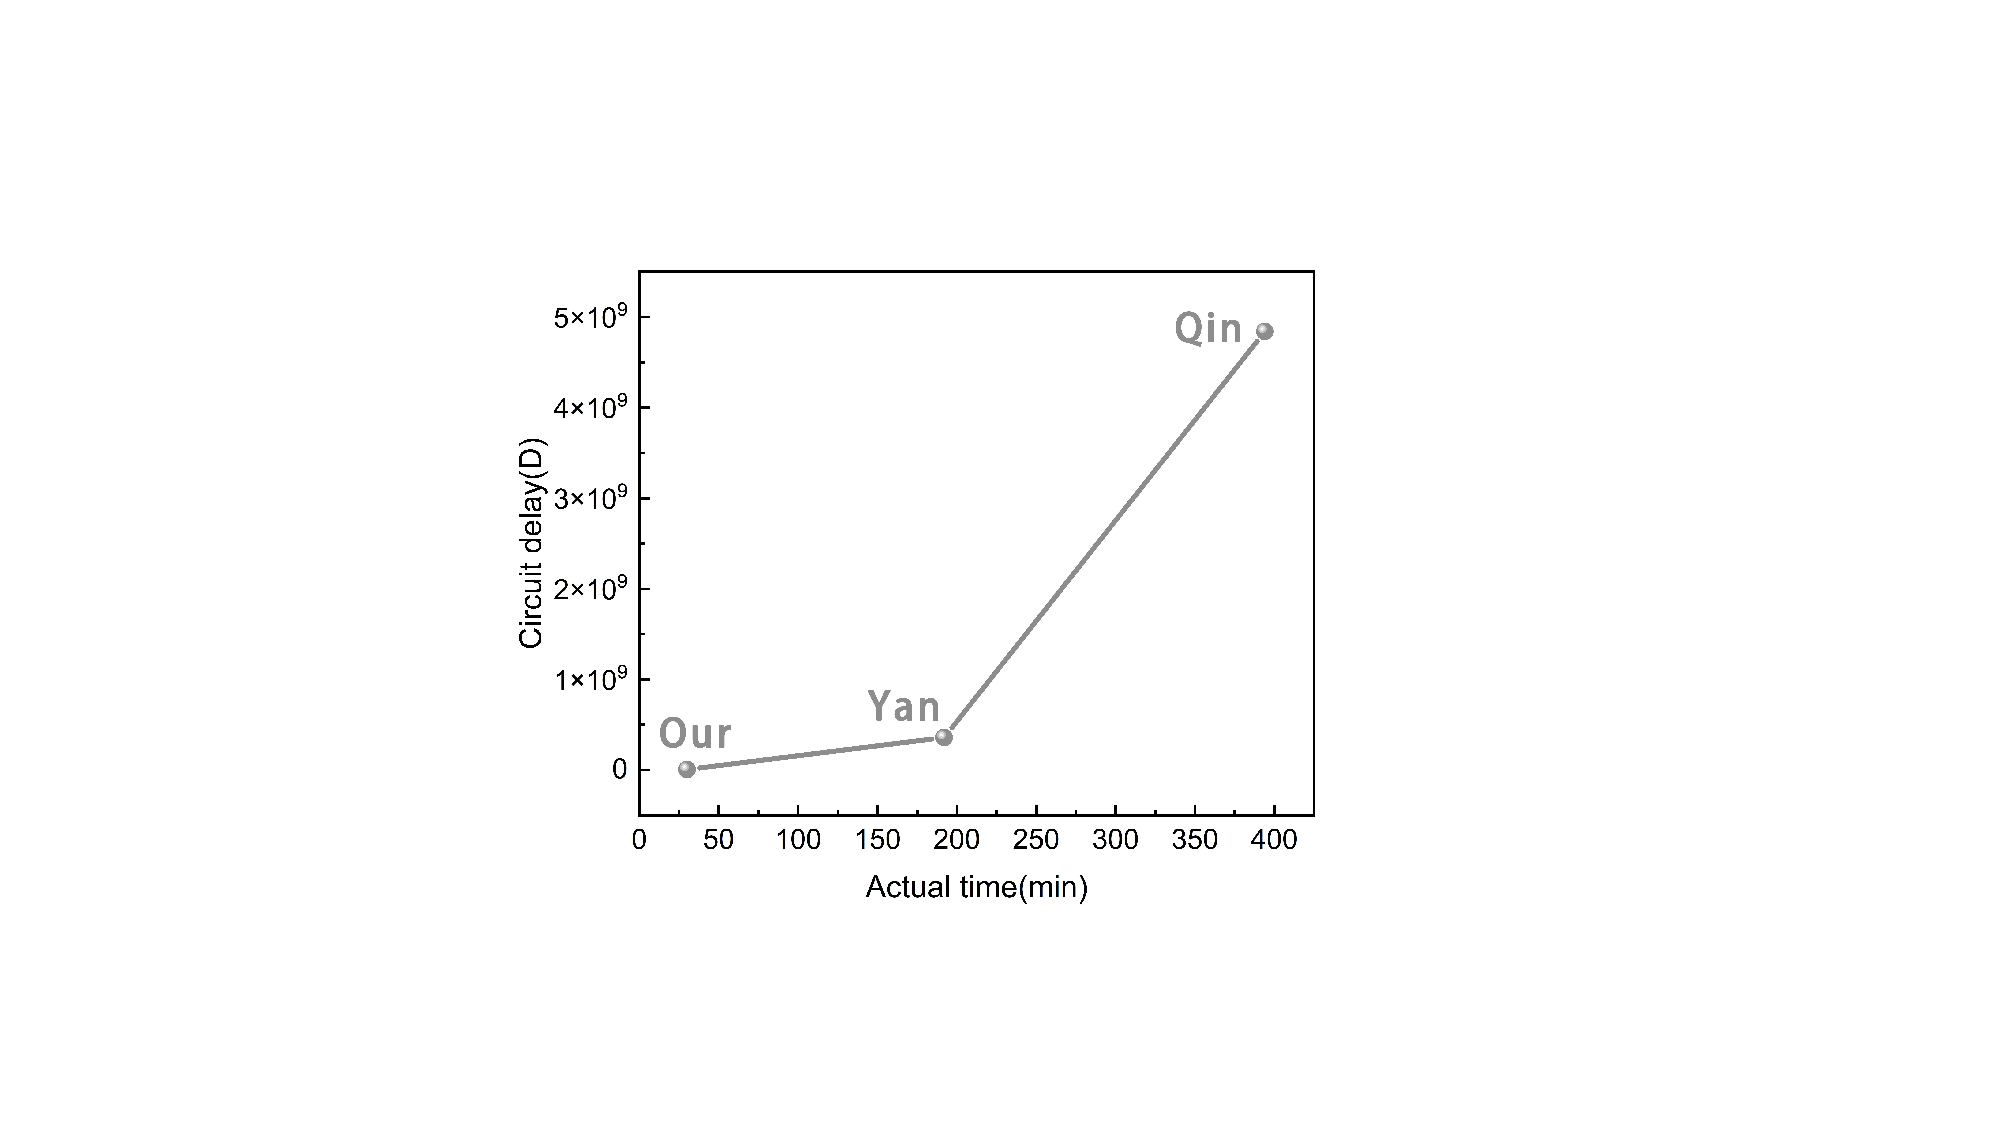
\includegraphics[width=1.8in]{4321.pdf}
		\end{minipage}
	}%
	\subfigure[\label{fig18(b)}]{
		\begin{minipage}[t]{0.5\linewidth}
			\centering
			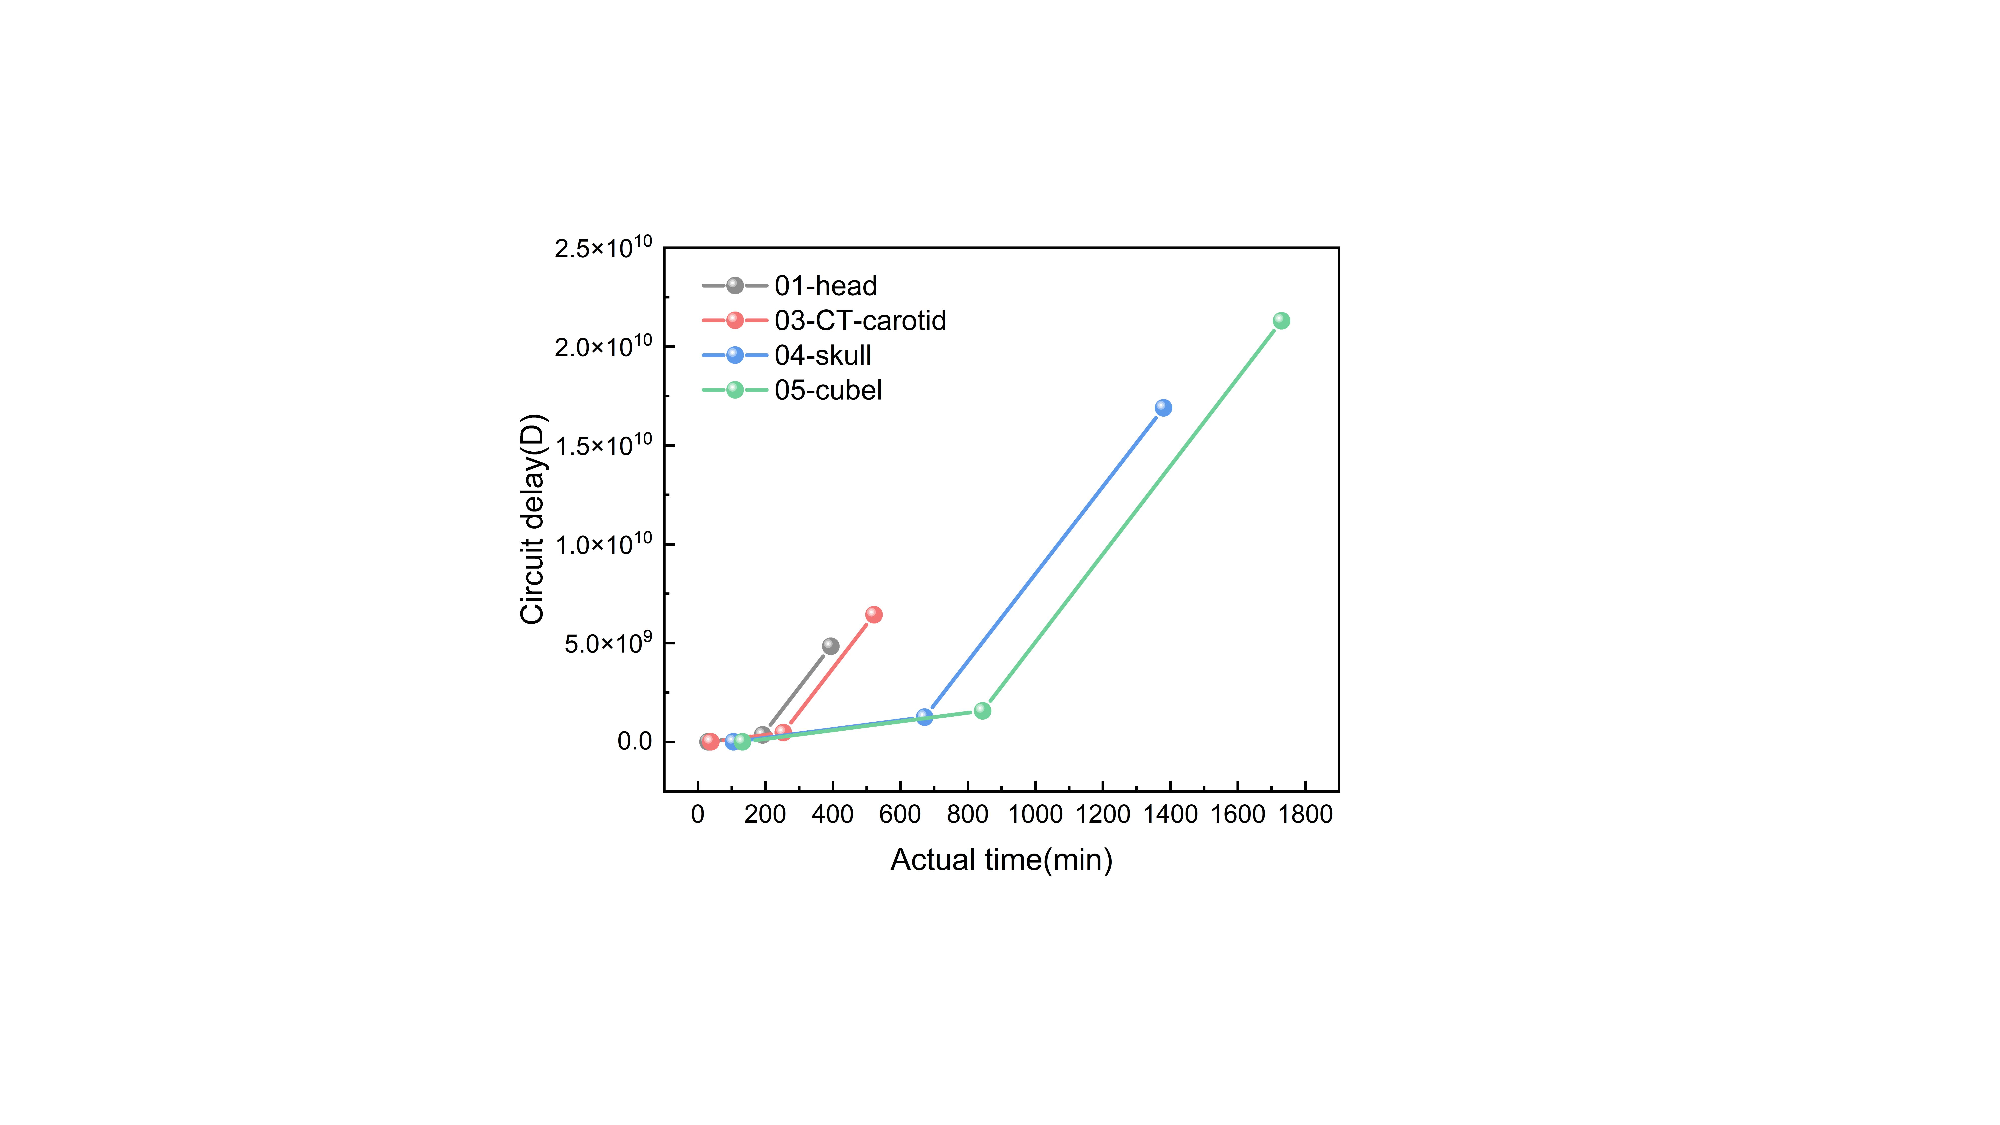
\includegraphics[width=1.8in]{1234.pdf}
		\end{minipage}
	}%
	\centering
	\caption{Actual time and circuit delay:(a)Experimental results of 01-head. (b)Experimental results of different 3D data cubes.}
	\label{fig18}
\end{figure}

As seen in Fig. \ref{fig18(a)}, the actual time is linearly related to the circuit delay. This shows that our scheme can indeed accelerate the secret sharing of 3D data cubes. It can be seen in Fig. \ref{fig18(b)}, our scheme has a great advantage when dealing with large data volumes of 3D data cubes.

\section{Conclusion}\label{Sec_conclusion}

In this paper, we apply secret sharing to 3D data cubes without key management while protecting image information. Also, the process is implemented on FPGA using parallelism, which greatly reduces the complexity of computation and improves the efficiency. Extending the process to multi-party computation achieves an efficient implementation of its four basic processes.

\begin{acknowledgements}
This work was funded by the Shandong Provincial Natural Science Foundation (No. ZR2021MF050), the MOE (Ministry of Education in China) Project of Humanities and Social Sciences (Project No. 18YJAZH110),  and the National Statistics Science Project (2021LY082).
\end{acknowledgements}


% Authors must disclose all relationships or interests that 
% could have direct or potential influence or impart bias on 
% the work: 
%
\section*{Conflict of interest}
\begin{itemize}
	\item Conflict of interest: The authors declare no competing interests.
	\item Data availability: The data used in this study are available from the corresponding author upon request.
	\item Authors' contributions: All authors contributed to the study conception and design. Material preparation, data collection and analysis were performed by[Tao Liu], [Bin Yan], [Jeng-Shyang Pan] and [Hong-Mei Yang]. The first draft of the manuscript was written by [Zi-Ming Wu] and all authors commented on previous versions of the manuscript. All authors read and approved the final manuscript.
	
\end{itemize}
%
% The authors declare that they have no conflict of interest.


% BibTeX users please use one of
%\bibliographystyle{spbasic}      % basic style, author-year citations
%\bibliographystyle{spmpsci}      % mathematics and physical sciences
\bibliographystyle{spphys}       % APS-like style for physics
\bibliography{sn-bibliography}% common bib file



\end{document}
% end of file template.tex

